\documentclass[11pt]{article}
\usepackage[T1]{fontenc}
\usepackage[utf8]{inputenc}
\usepackage{lmodern}
\usepackage[margin=1in]{geometry}
\usepackage{amsmath,amssymb,amsthm,mathtools,bm}
\usepackage{booktabs,array,tabularx}
\usepackage{graphicx}
\usepackage[font=small,labelfont=bf]{caption}
\usepackage{setspace}
\usepackage{microtype}
\usepackage[hidelinks]{hyperref}
\urlstyle{same}
\usepackage[section]{placeins}
\onehalfspacing
\setlength{\emergencystretch}{2em}
\DeclareMathOperator{\tr}{tr}
\DeclareMathOperator{\diag}{diag}
\DeclareMathOperator{\KL}{KL}
\DeclareMathOperator{\TC}{TC}
\DeclareMathOperator{\Var}{Var}
\DeclareMathOperator{\Cov}{Cov}
\newcolumntype{L}{>{\raggedright\arraybackslash}X}
\graphicspath{{figures/}}
\newtheorem{theorem}{Theorem}
\newtheorem{proposition}{Proposition}
\newtheorem{lemma}{Lemma}
\newtheorem{corollary}{Corollary}
\numberwithin{equation}{section}
\hypersetup{
  pdftitle={Fitting One Factor to Two Traits: Population Solutions and Fit Indices},
  pdfauthor={},
  pdfsubject={Manuscript submitted to Psychometrika}
}

\title{Fitting One Factor to Two Traits:\\Population Solutions and Fit Indices}
% Default build: anonymised for review; author details are on the separate
% cover page (cover_page.tex). Built with \def\preprint{} (see build.py),
% this file gives the named preprint with its declarations.
\ifdefined\preprint
  % Named front matter for the preprint: main.tex built with \def\preprint{}
% (see build.py). The anonymised manuscript does not load this file.
% Author details shared by the cover page (cover_page.tex) and the named
% preprint (preprint_front.tex). Edit them here only. The anonymised
% manuscript (main.tex in its default build) does not load this file.
\newcommand{\AuthorName}{Aleksandar Tomašević}
\newcommand{\AuthorAffiliation}{Institute of Physics Belgrade, University of Belgrade, Serbia}
\newcommand{\AuthorEmail}{atomashevic@gmail.com}
\newcommand{\AuthorORCID}{0000-0003-4863-6051}

\author{\AuthorName\\[2pt]
  {\small \AuthorAffiliation}\\
  {\small \href{mailto:\AuthorEmail}{\AuthorEmail}\quad ORCID: \AuthorORCID}}
\date{Preprint, version 1}
\hypersetup{pdfauthor={\AuthorName}, pdfsubject={Preprint}}

\else
  \author{}
  \date{}
\fi
\begin{document}
\maketitle
\begin{abstract}
A one-factor model fitted to items from two correlated traits need not represent both traits equally. We characterize its population maximum likelihood solution and derive the resulting fit indices. For two equal blocks of $m$ items with loading $\lambda$, the optimal solution represents an equal composite when the trait correlation is at least $\varphi^* = (1 + (m-1)\lambda^2)/(m(2-\lambda^2))$. Below this threshold, two equally good solutions favor different traits; at zero correlation, each represents one trait alone. For this design, we establish global optimality over the unrestricted one-factor model and extend the analysis to unequal blocks and least-squares estimation. The solutions give exact population CFI, TLI, RMSEA, and SRMR, including the trait correlations at which conventional cutoffs are met. With loadings of .7 and 4 to 16 items in total, CFI reaches .95 at correlations of .78 to .84, although two traits generate the data. Numerical studies examine binary and ordinal items and finite samples. They also show that item order can change the solution returned by lavaan's default starting values. The results provide design-specific benchmarks for interpreting one-factor fit and for assessing which traits the fitted factor represents.
\par\medskip
\noindent\textbf{Keywords:} factor analysis, fit indices, model misspecification, unidimensionality, symmetry breaking
\end{abstract}

\section{Introduction}
\label{sec:introduction}

A one-factor model fitted to items from two correlated traits can represent both traits equally or primarily one of them. The optimal representation depends on the trait correlation, the loadings, the number of items, and the estimator. Global fit addresses a different property: how closely the fitted model reproduces the item correlations. Consequently, neither acceptable fit nor the decision to fit one factor establishes that the factor represents both traits equally. We characterize the population one-factor solution in a two-block design, derive its fit indices, and determine the trait correlations at which conventional cutoffs are met.

The distinction matters for scales that combine related domains, such as the PHQ-ADS, which sums the nine depression items of the PHQ-9 and the seven anxiety items of the GAD-7. In its validation, the estimated depression--anxiety correlations were .912, .865, and .653 in three trials, and the one-factor model met the CFI cutoff of .95 in the first two trials but exceeded the RMSEA cutoff of .06 in all three. Kroenke et al.\ (2016) retained the total score on the basis of additional evidence, including bifactor indices and scree plots. Such a result leaves two issues to resolve: whether the fit criteria can distinguish the two-trait structure from a single factor, and whether the fitted factor gives comparable weight to depression and anxiety.

The same issues arise when two constructs are merged into one factor whose fit is compared with that of a two-factor model to assess whether they are distinct (R\"onkk\"o \& Cho, 2022), and in unidimensional item response theory (IRT), where a single ability is estimated from items that may depend on more than one trait (Ackerman, 1989; Reckase, 1979). In these settings, CFI, RMSEA, and SRMR are often interpreted with conventional cutoffs (Hu \& Bentler, 1999), although the performance of a cutoff depends on the model and the form of misspecification (McNeish \& Wolf, 2023).

Our main result identifies when the best one-factor approximation treats the two traits equally. Suppose that each trait has $m$ indicators, all with standardized loading $\lambda$, and that errors are independent. Under normal-theory maximum likelihood (ML), the optimal solution has equal loadings on both item blocks when the trait correlation is at least
\[
\varphi^*=\frac{1+(m-1)\lambda^2}{m(2-\lambda^2)}.
\]
Below this correlation, two optimal solutions with identical fit have larger loadings on one block than on the other, because either trait can receive the larger weight. At zero correlation, the factor reproduces one block exactly and assigns zero loadings to the other. We refer to the equal-loading solution as the \emph{composite solution} and to the unequal-loading solutions as \emph{tilted solutions}; Figure~\ref{fig:1} shows both for four items per trait with loading .7. The change between them is a symmetry-breaking transition: the population is unchanged when the two item blocks are exchanged, but an optimal fitted model below the threshold is not. We establish the global minimum on both sides of the transition, rather than only comparing selected stationary solutions. As in Cudeck and Browne's (1992) analysis of covariance-model misspecification, this approximation problem is defined in the population, before sampling variability is introduced.

The minimum discrepancy also gives exact population CFI, TLI, RMSEA, and SRMR. Kenny and McCoach (2003, pp.~342--345) derived the symmetric fitted covariance and its population CFI and TLI for the two-trait design considered here. For this design, we determine when the symmetric solution is globally optimal and obtain the optimum when it is not, so that the resulting cutoff boundaries use the global minimum throughout the correlation range. For example, with loadings of .7 and 4 to 16 items in total, CFI reaches .95 when the traits correlate .78 to .84. These correlations lie above the transition, so the approximation that meets the CFI criterion here is a composite of two traits; the distinction between dimensionality, global fit, and trait representation remains necessary in both regimes.

When two equally long blocks have different loadings, the global ML solution favors the block with higher loadings, but a second local minimum can favor the other trait. We derive an exact condition for this second minimum and characterize the sensitivity to small loading differences near the symmetric threshold. Unequal block lengths can also change which trait receives greater weight. The estimator matters independently of these design differences: for the exchangeable design, the transition under unweighted least squares occurs at $1/p$, where $p$ is the total number of items, and the weighted least-squares result explains why a composite solution persists to still lower correlations in the ordinal designs examined here. Finally, the population minimum discrepancy does not depend on item order, but an optimizer's starting values can. Our finite-sample study, conducted with lavaan (Rosseel, 2012) in R (R Core Team, 2025), shows that this dependence can change both the returned loading pattern and its discrepancy; in unequal-block designs, the returned solution can favor the weaker block and fit worse than a solution obtained from another start.

This analysis relates to three strands of previous work. First, studies of unidimensional IRT often describe the fitted ability as an average or reference composite of the generating traits (Ackerman, 1989; Ansley \& Forsyth, 1985), and Strachan et al.\ (2022) reported agreement with a linear composite conjecture for nonnegative trait correlations but instability at negative correlations. These findings concern particular item structures and estimators. Our analysis identifies an explicit transition for a two-block population and shows how common cross-loadings change the relevant correlation, providing a mechanism for different one-factor representations without assuming that all multidimensional item sets have the same unidimensional approximation. Second, fit indices depend on the measurement design: higher loadings can produce poorer fit at a fixed misspecification, a result described as the reliability paradox (Hancock \& Mueller, 2011; Heene et al., 2011; McNeish et al., 2018), and more items can move CFI and RMSEA in different directions (Kenny \& McCoach, 2003; Shi et al., 2019). Groskurth et al.\ (2024) examined one-factor fits to two-factor ordinal data, showed that fit-index behavior depends on the estimator and measurement design, and discussed how omitted cross-loadings can change the meaning of fitted factors in a two-factor model despite apparently good fit. Groskurth et al.\ (2025) used a two-factor alternative to a one-factor model in their simulation-cum-ROC approach to selecting fit indices and cutoffs. The present analysis complements these studies by characterizing the minimizing covariance and its trait representation for a specified two-block population. Third, Fukasaku et al.\ (2025) developed algebraic methods for enumerating ML candidates and illustrated changes in the configuration of minima; the present population analysis gives a global classification for the exchangeable design and explicit conditions for competing minima when equally long blocks have different loadings.

Appendices~\ref{app:ml}--\ref{app:ceiling} give the proofs or their main steps, Appendix~\ref{supp:numerical} documents the numerical study, Appendix~\ref{app:binary} treats binary items, and Online Resources 1--3 give the complete proofs.

\section{Population Model and Measures of Fit}
\label{sec:setup}

Consider two standardized traits, $\theta_1$ and $\theta_2$, with correlation $\varphi\in[0,1)$. Block A contains $m\ge2$ items that load only on $\theta_1$, and block B contains $m$ items that load only on $\theta_2$, so the test has $p=2m$ items. Every item has standardized loading $\lambda\in(0,1)$ and an independent error with variance $1-\lambda^2$. The population correlation matrix $R$ has unit diagonal, within-block correlations $\lambda^2$, and between-block correlations $\lambda^2\varphi$. We write $R_A$ and $R_B$ for the within-block correlation matrices of blocks A and B, that is, the two diagonal blocks of $R$. Negative trait correlations are obtained by reflecting one block. The minimization results depend on the population only through its correlation matrix $R$. Normality is assumed only to give the ML discrepancy its likelihood and information interpretations.

We fit the unrestricted one-factor covariance model
\[
\Sigma=ll^{\top}+\Psi,\qquad
\Psi=\diag(\psi_1,\ldots,\psi_p),\qquad
\psi_i\ge0,\quad \Sigma\succ0.
\]
In particular, equality of the fitted loadings or uniquenesses is not imposed. The population maximum likelihood discrepancy is
\begin{equation}
F(\Sigma)=\tr(\Sigma^{-1}R)-\log\det(\Sigma^{-1}R)-p,
\label{eq:ml-discrepancy}
\end{equation}
and $F_{\min}$ denotes its minimum over this model. The independence model has discrepancy $F_B=-\log\det R$. The population fit indices are
\begin{equation}
\begin{aligned}
\mathrm{CFI}&=1-\frac{F_{\min}}{F_B},&
\mathrm{TLI}&=1-\frac{F_{\min}/\mathit{df}_M}{F_B/\mathit{df}_B},&
\mathrm{RMSEA}&=\sqrt{\frac{F_{\min}}{\mathit{df}_M}},
\end{aligned}
\label{eq:population-indices}
\end{equation}
where $\mathit{df}_M=p(p-3)/2$ and $\mathit{df}_B=p(p-1)/2$. SRMR is the root mean square residual correlation over the $p(p+1)/2$ nonredundant matrix entries, including the diagonal. These are population quantities: they depend only on $R$ and the fitted covariance, not on sample size. The sample indices reported in Section~\ref{sec:numerical} estimate them, with the usual truncation at zero for noncentrality-based indices.

These indices summarize different aspects of the same approximation. Under normality, $F(\Sigma)=2\KL\{\mathcal N(0,R)\,\|\,\mathcal N(0,\Sigma)\}$ (Akaike, 1987), whereas $F_B=2\TC(R)$ is twice the total correlation, or multi-information, among the items; for a correlation matrix $S$, $\TC(S)=-\tfrac12\log\det S$ (Watanabe, 1960). CFI therefore expresses the reduction in this information loss relative to independence. RMSEA expresses the square root of the loss per model degree of freedom. Their denominators differ, so their judgments of the same fitted covariance need not agree (Lai \& Green, 2016).

At an ML solution of a scale-invariant covariance model, $\tr(\hat\Sigma^{-1}R)=p$ (Dijkstra, 1990). Consequently,
\begin{equation}
F_{\min}=\log\det\hat\Sigma-\log\det R.
\label{eq:entropy-gap}
\end{equation}
Appendix~\ref{app:entropy} interprets this difference in terms of Gaussian entropies. All solutions considered here also reproduce the item variances. For these solutions, population CFI equals $\TC(\hat\Sigma)/\TC(R)$, the fraction of the population multi-information present in the fitted covariance. Equivalently, it is the ratio of the two log determinants (Kenny \& McCoach, 2003, Eq.~10). These established identities provide an interpretation of the results below; the new question is which one-factor covariance minimizes the discrepancy.

For the equal-block design, write
\[
L=\lambda^2,\qquad a=1-L,\qquad n=m-1,\qquad
\nu =2m-1,\qquad b=1+nL,
\]
and set $h=mL\varphi$ and $q=h/b$. The eigenvalues of $R$ are $a$, with multiplicity $2n$, and $b+h$ and $b-h$, corresponding to the sum and difference of the block means. Hence
\[
\det R=a^{2n}b^2(1-q^2).
\]
The quantity $\kappa_-=mL(1-\varphi)/a$ is the signal-to-noise ratio for the contrast between the traits: the difference eigenvalue is $b-h=a(1+\kappa_-)$, with signal part $mL(1-\varphi)$ and noise part $a$. We also use $F_0=-n\log a-\log b=-\log\det R_A=2\TC(R_A)$, the independence-model discrepancy of a single block, and $q^*=L/(2-L)$, the value of $q$ at the threshold $\varphi^*$ of Theorem~\ref{thm:ml}. Because $q$ increases with $\varphi$, the condition $\varphi\ge\varphi^*$ is equivalent to $q\ge q^*$.

\section{The Population Maximum Likelihood Solution}
\label{sec:ml-classification}

The best one-factor approximation need not give equal weight to equally measured traits. When the traits are sufficiently correlated, maximum likelihood produces equal fitted loadings across the two blocks. Below a calculable threshold, two equally good solutions replace this composite: one has larger loadings on block A and the other on block B. The following result gives the threshold and characterizes the solutions over the unrestricted model.

\begin{theorem}[Maximum likelihood solution]
\label{thm:ml}
Under the population model in Section~\ref{sec:setup}, define
\begin{equation}
\varphi^*=\frac{1+(m-1)\lambda^2}{m(2-\lambda^2)}=\frac{b}{m(2-L)}.
\label{eq:ml-threshold}
\end{equation}
The ML discrepancy attains its minimum. For $\varphi\ge\varphi^*$, the minimizing covariance is unique. Up to a common sign, all fitted loadings equal $l_s$, where
\[
l_s^2=\frac{L(n+m\varphi)}{\nu },\qquad \psi_i=1-l_s^2.
\]
For $0<\varphi<\varphi^*$, there are exactly two minimizing covariances, interchanged by exchanging the blocks. After choosing a common positive sign and the block order, their fitted loadings are $\alpha>\beta>0$, constant within each block, with
\begin{equation}
\alpha\beta=q,\qquad
\alpha^2+\beta^2=L+(2-L)q^2,
\label{eq:ml-asymmetric-loadings}
\end{equation}
and their uniquenesses are $1-\alpha^2$ in block A and $1-\beta^2$ in block B.
At $\varphi=0$, each minimizing covariance reproduces one population block exactly and replaces the other by an identity matrix, so the other block has zero loadings and unit uniquenesses. For $m\ge3$, the retained block has loadings $\lambda$ and uniquenesses $a$, up to a common sign. For $m=2$, up to a common sign, the retained loadings may be $(t,L/t)$ for any $L\le t\le1$, with uniquenesses $(1-t^2,1-L^2/t^2)$. All such representations give the same covariance for the retained block; the endpoints each have one zero uniqueness. There are two minimizing covariances, one for each choice of retained block.

For every $0<\varphi<1$, every local minimum over the full feasible model is global. The symmetric stationary point, with all loadings equal to $l_s$ as defined above, is a saddle for $0\le\varphi<\varphi^*$. The minimum discrepancy is
\begin{equation}
F_{\min}(\varphi)=
\begin{cases}
F_0+n\log(1-q^2),&0\le\varphi\le\varphi^*,\\[3pt]
\nu \log\!\left(1+\dfrac{\kappa_-}{\nu }\right)-\log(1+\kappa_-),
&\varphi^*\le\varphi<1.
\end{cases}
\label{eq:ml-minimum}
\end{equation}
The two expressions agree at $\varphi^*$.
\end{theorem}

The second form shows that $\varphi^*$ is the trait correlation at which $q=q^*$ (Section~\ref{sec:setup}). The behavior of the solution as $\varphi$ approaches this threshold follows from the closed forms in Theorem~\ref{thm:ml}.

\begin{corollary}[Behavior at the transition]
\label{cor:ml-transition}
Under the conditions of Theorem~\ref{thm:ml}, $F_{\min}$ is continuous on $[0,1)$ and real analytic away from $\varphi^*$. At $\varphi^*$, $F_{\min}$ is continuously differentiable but not twice continuously differentiable, and the symmetric solution is the unique minimizer although the discrepancy has zero curvature in the symmetry-breaking direction and grows quartically along it. For $0<\varphi<\varphi^*$, the loading difference satisfies
\begin{equation}
(\alpha-\beta)^2=(2-L)(q^*-q)(1-q),
\label{eq:loading-gap}
\end{equation}
and therefore, as $\varphi\uparrow\varphi^*$,
\[
|\alpha-\beta|\sim
\lambda\sqrt{\frac{2m(1-\lambda^2)}{1+(m-1)\lambda^2}}
(\varphi^*-\varphi)^{1/2}.
\]
\end{corollary}

The complete proof of Theorem~\ref{thm:ml} is given in Online Resource~1. Appendix~\ref{app:ml} presents its main reductions. The argument first establishes existence and excludes boundary minima by a zero-uniqueness criterion (Proposition~\ref{prop:boundary}, Appendix~\ref{app:heywood-proof}), apart from the stated two-item endpoint representations. It then shows that every local minimum at positive trait correlation has constant loadings within each block. Minimization of a one-dimensional profile completes the global comparison. Thus the conclusion does not depend on imposing equal fitted loadings or on examining the Hessian at the symmetric solution alone. Appendix~\ref{app:ml} also gives the second-derivative jump at $\varphi^*$ and the local expansion behind Corollary~\ref{cor:ml-transition}.

The substantive distinction is between an equal composite and a factor that gives greater weight to one trait. Above $\varphi^*$, the fitted covariance has equal uniquenesses, and its discrepancy is the familiar maximum likelihood expression for a one-factor model with equal uniquenesses, the probabilistic principal component model: $p-1$ times the logarithm of the ratio of the arithmetic and geometric means of the $p-1$ nonleading eigenvalues of $R$ (Lawley, 1956; Tipping \& Bishop, 1999). Kenny and McCoach (2003, pp.~342--345) give the same symmetric fitted covariance and the corresponding CFI and TLI. Theorem~\ref{thm:ml} establishes when that covariance is the unrestricted optimum. Below $\varphi^*$, the symmetric expression overstates the minimum discrepancy because the optimum has unequal block loadings.

The threshold can occur at a substantial trait correlation. With loadings of .7 and four items per trait, $\varphi^*=.409$ (Figure~\ref{fig:1}). At lower correlations the population itself admits two equally good, substantively different one-factor solutions. This ambiguity exists before sampling error or numerical optimization enters the problem. It concerns the fitted measurement model; the trait composition of an estimated factor score is a separate quantity, considered in Section~\ref{sec:unequal}.

The result also gives a simple reference value for comparative fit. At $\varphi=0$, $F_{\min}=F_0$ and $F_B=2F_0$, so population CFI is exactly $1/2$ for every admissible loading and block size. One factor retains all the multi-information in one block and none in the other. Throughout the asymmetric regime,
\begin{equation}
\mathrm{CFI}_{\mathrm{pop}}
=1-\frac{F_0+n\log(1-q^2)}{2F_0-\log(1-q^2)},
\qquad 0\le\varphi\le\varphi^*.
\label{eq:cfi-asymmetric}
\end{equation}
The next section uses this global solution to determine what conventional fit criteria imply about the underlying two-trait population.

\begin{figure}[t]
\centering
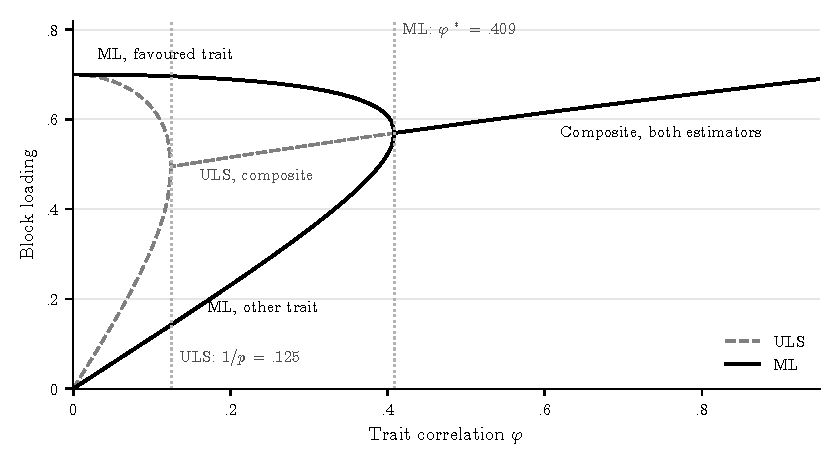
\includegraphics[width=0.85\textwidth]{fig1.pdf}
\caption{Fitted block loadings for two traits measured by four items each, with population loading .7. The ML solution has unequal block loadings below $\varphi^*=.409$. The ULS solution remains symmetric down to $\varphi=1/p=.125$; its characterization is given in Theorem~\ref{thm:uls}. Solid lines represent ML and dashed lines represent ULS. Both estimators give the same symmetric fitted covariance above the ML threshold and retain one trait at zero correlation.}
\label{fig:1}
\end{figure}

\section{Population Fit and the Distinction Between Traits}
\label{sec:fit-indices}

The minimum discrepancy in Theorem~\ref{thm:ml} provides a population benchmark for interpreting a one-factor fit. For a specified loading and test length, it identifies the trait correlations at which the fitted model meets a conventional cutoff although two traits generated the data. These cutoff boundaries concern overall fit. The threshold $\varphi^*$ concerns which direction the fitted factor represents. The two boundaries answer different questions.

\subsection{Cutoff Boundaries}

Table~\ref{tab:1} gives the cutoff boundaries for CFI, TLI, RMSEA and SRMR. With loadings of .70 and 4 to 16 items in total, a one-factor model meets CFI $\ge .95$ when the trait correlation reaches approximately .78 to .84. The corresponding RMSEA boundary decreases from .92 to .84 as items are added. Thus, a favorable CFI does not establish that the two generating traits are identical, and disagreement between indices can occur at the population level.

\begin{table}[t]
\centering\small
\caption{Trait-correlation boundaries for conventional population fit cutoffs. Each entry is the trait correlation, calculated from Theorem~\ref{thm:ml} and rounded to two decimals, at which the population index reaches the cutoff. In each tabled design, each index is monotone in $\varphi$ (checked numerically on a grid of step .01), so each boundary is a single crossing and the cutoff is met at all larger correlations. The item count is $p=2m$. ``Many'' gives the limit as $m\to\infty$: CFI and TLI from $\mathrm{CFI}_\infty$, SRMR from $\lambda^2(1-\varphi)/2$, and population RMSEA tends to zero for every $\varphi$. ``Any $\varphi$'' indicates that the cutoff is met throughout $0\le\varphi<1$. The final column gives the ML threshold $\varphi^*$ for equal versus unequal fitted loadings across the two blocks; its ``many'' entry is the limit $\lambda^2/(2-\lambda^2)$.}
\label{tab:1}
\begin{tabular}{ccccccc}
\toprule
Loading & Total items & CFI $\ge .95$ & TLI $\ge .95$ & RMSEA $\le .06$ & SRMR $\le .08$ & ML $\varphi^*$ \\
\midrule
.50 & 4 & .71 & .83 & .76 & any $\varphi$ & .36 \\
.50 & 8 & .74 & .78 & .64 & .27 & .25 \\
.50 & 16 & .77 & .79 & .54 & .32 & .20 \\
.50 & many & .91 & .91 & any $\varphi$ & .36 & .14 \\
.70 & 4 & .78 & .87 & .92 & .55 & .49 \\
.70 & 8 & .82 & .85 & .88 & .63 & .41 \\
.70 & 16 & .84 & .86 & .84 & .65 & .37 \\
.70 & many & .93 & .93 & any $\varphi$ & .67 & .32 \\
.85 & 4 & .86 & .92 & .97 & .70 & .67 \\
.85 & 8 & .88 & .91 & .95 & .75 & .62 \\
.85 & 16 & .90 & .91 & .94 & .76 & .59 \\
.85 & many & .95 & .95 & any $\varphi$ & .78 & .57 \\
\bottomrule
\end{tabular}
\end{table}

All of the CFI $\ge .95$ boundaries in Table~\ref{tab:1} lie in the equal-loading regime of Theorem~\ref{thm:ml}. Consequently, these examples of favorable CFI should be distinguished from the preferential representation of one trait at lower correlations. The practical point is that an overall fit index does not by itself resolve either the dimensionality of the population or the interpretation of the fitted factor.

The closed forms for CFI, TLI and RMSEA follow by substituting $F_{\min}$ into their definitions. For SRMR, the fitted model reproduces the diagonal, and the remaining residuals take three values. Hence
\[
\mathrm{SRMR}^2=
\frac{\tfrac{m(m-1)}{2}\big[(L-\alpha^2)^2+(L-\beta^2)^2\big]+m^2(L\varphi-\alpha\beta)^2}
{m(2m+1)}.
\]
In the equal-loading regime, this reduces to
\[
\mathrm{SRMR}
=\lambda^2(1-\varphi)\sqrt{\frac{m(m-1)}{4m^2-1}}
\;\longrightarrow\;\frac{\lambda^2(1-\varphi)}{2}.
\]
For $\varphi\ge\lambda^2/(2-\lambda^2)$, the limiting CFI and TLI as the number of items increases are
\[
\mathrm{CFI}_{\infty}=\mathrm{TLI}_{\infty}
=1-\frac{\log\big(1+\lambda^2(1-\varphi)/[2(1-\lambda^2)]\big)}
{-\log(1-\lambda^2)}.
\]

The indices differ because they summarize discrepancy in different ways. RMSEA divides the discrepancy by the model degrees of freedom. It decreases at rate $m^{-1/2}$ for fixed loading and trait correlation, and its limit is zero. Thus, sufficiently long tests meet a fixed positive RMSEA cutoff even when the two traits are uncorrelated. CFI and TLI compare model discrepancy with independence-model discrepancy; TLI also adjusts for degrees of freedom. At loading .70, their limiting .95 cutoff boundary is approximately .93. Finite-length boundaries need not be monotone: the TLI boundaries are .87, .85 and .86 for 4, 8 and 16 items.

SRMR instead summarizes the sizes of residual correlations. It depends directly on $\lambda^2$ and has little dependence on test length once $m$ is moderately large. It does not normalize residuals by their precision or by baseline discrepancy. It is the most permissive cutoff for the finite item counts in Table~\ref{tab:1}. For four items loading .50, SRMR is .079 at $\varphi=0$, so two independent traits meet the .08 cutoff.

Kenny and McCoach (2003) derived the symmetric-branch population CFI and TLI. The limiting expression above follows from their determinant formulas, and they also described the decline of RMSEA with test length. Shi, Lee and Maydeu-Olivares (2019) studied model-size effects numerically. Theorem~\ref{thm:ml} adds the global classification: it identifies when the symmetric expression is the minimum and supplies the asymmetric branch when it is not. The cutoff calculations therefore use the minimum over the full one-factor model.

The exact discrepancy can also be used in the conventional noncentral-$\chi^2$ power approximation, with noncentrality $NF_{\min}$ for sample size $N$ under the normal-likelihood convention. This approximation is justified under regular local alternatives. Its finite-sample accuracy under fixed misspecification, near $\varphi^*$ and at nonregular endpoints is not established by the population formulas (Chun \& Shapiro, 2009).

\subsection{CFI at a Fixed Information Loss}

A change in CFI need not indicate a change in the information lost by the one-factor approximation. Fix $p=2m$ and the contrast signal-to-noise ratio $\kappa_-$, and vary the loading along
\[
\varphi=1-\frac{\kappa_-(1-\lambda^2)}{m\lambda^2},
\]
within the regime $\varphi\ge\varphi^*$. Theorem~\ref{thm:ml} implies that $F_{\min}$, the Kullback--Leibler divergence and RMSEA are constant on this path. The baseline discrepancy increases with $\lambda^2$, however, so CFI increases.

More explicitly, the derivative of total correlation with respect to $\lambda^2$ along this path is positive exactly when
$\kappa_-<(2m-1)\lambda^2/(1-\lambda^2)$, a condition satisfied on the stated path with $\varphi\ge0$. For eight items and $\kappa_-=1$, the Kullback--Leibler divergence is .121 (half of $F_{\min}=.242$) and RMSEA is .110 throughout the path, whereas CFI is .62, .82, .91, .95 and .97 at loadings .5, .6, .7, .8 and .9. At loading .5 the path meets the threshold, $\varphi=\varphi^*=.25$.

Moshagen and Auerswald (2018) showed that RMSEA and the conventional noncentral-$\chi^2$ power approximation do not depend on loadings when discrepancy is held fixed. The calculation here gives the corresponding result for an incremental index. It also clarifies the relation to the reliability paradox: studies of that phenomenon hold the form of misspecification fixed and find that fit worsens as loadings increase (Hancock \& Mueller, 2011; McNeish, An \& Hancock, 2018). The direction of the loading effect depends on which feature of the population is held constant.

For heterogeneous loadings, the exact expressions need not apply. Proposition~\ref{prop:ceiling} in Appendix~\ref{app:ceiling} gives an upper bound on the information lost by the best one-factor approximation. The bound depends on the smaller eigenvalue of the trait signal after each item is scaled by its unique standard deviation.

\section{Estimation Criteria and Unequal Measurement}
\label{sec:extensions}

The exchangeable ML solution provides a benchmark. We next examine how that benchmark changes with the fitting criterion, differences between item blocks, and cross-loadings. These extensions separate the effects of the estimator from the effects of the measurement design.

\subsection{Dependence on the Fitting Criterion}
\label{sec:estimators}

The transition in Theorem~\ref{thm:ml} depends on the estimation criterion. Under unweighted least squares (ULS), it occurs at $1/p$, independently of the population loading. Principal components retain the equal block-mean direction at every positive trait correlation. Thus a single population can yield an equal composite under one criterion and a factor that emphasizes one trait under another.

\begin{theorem}[Unweighted least squares solution]
\label{thm:uls}
For the population in Section~\ref{sec:setup}, let
\[
G(l)=\sum_{i<j}(R_{ij}-l_il_j)^2,\qquad |l_i|\le1,
\]
be the least-squares, or MINRES, objective with free uniquenesses; the constraint $|l_i|\le1$ is equivalent to $\psi_i=1-l_i^2\ge0$. For $\varphi>0$, every global minimizer has a common loading sign. Choose that sign to be positive. If $0<\varphi<1/(2m)=1/p$, every global minimizer is constant within blocks; after ordering the blocks, its block loadings $\alpha>\beta>0$ satisfy
\[
\alpha^2+\beta^2=L,\qquad \alpha\beta=mL\varphi,
\qquad
G_{\min}=\frac{m(m-1)L^2}{2}-m^2(m-1)L^2\varphi^2.
\]
At and above $\varphi=1/(2m)$, the positive minimizer is unique and symmetric, with
\[
l^2=\frac{L(n+m\varphi)}{\nu },\qquad
G_{\min}=\frac{m^2(m-1)L^2(1-\varphi)^2}{2m-1}.
\]
The branches coincide at $\alpha^2=\beta^2=L/2$. For $0<\varphi\le1/(2m)$,
\[
|\alpha-\beta|=\lambda\sqrt{2m}\sqrt{\frac1{2m}-\varphi}.
\]
At $\varphi=0$, either block is fitted exactly and the other has zero loadings, giving $G_{\min}=m(m-1)L^2/2$. For $m\ge3$, all retained loadings equal $\lambda$, up to their common sign. For $m=2$, the retained pair is $(t,L/t)$, $L\le t\le1$, up to its common sign; these representations give the same retained-block covariance.

\end{theorem}

Appendix~\ref{app:uls} outlines the unrestricted proof. The argument uses a tight relaxation to establish constant loadings within blocks, then minimizes a convex quadratic over a cone. The result characterizes global minimizers; it does not assert a complete classification of nonglobal ULS local minima.

Weighted least squares makes the source of the difference more explicit. Let $w_W>0$ and $w_C>0$ be the weights given to within-block and cross-block residual correlations, respectively, and define
\[
G_w(l)=w_W\sum_{\mathrm{within}}(R_{ij}-l_il_j)^2
+w_C\sum_{\mathrm{across}}(R_{ij}-l_il_j)^2,
\qquad \omega=\frac{w_C}{w_W}.
\]
Each weight is constant within its pair class.

\begin{proposition}[Weighted least squares solution]
\label{cor:wls}
For the population in Section~\ref{sec:setup}, minimize $G_w$ over $|l_i|\le1$. For $\varphi>0$, choose the common loading sign to be positive. If $\omega>(m-1)/m$, the threshold is
\begin{equation}
\varphi_\omega=\frac12-\frac{m-1}{2m\omega}.
\label{eq:wls-threshold}
\end{equation}
For $0<\varphi<\varphi_\omega$, every global minimizer is constant within blocks; after ordering the blocks, its block loadings $\alpha>\beta>0$ satisfy
\[
\alpha^2+\beta^2=L,\qquad
\alpha\beta=\frac{\omega mL\varphi}{\omega m-m+1}.
\]
At and above the threshold, the positive minimizer is unique and symmetric, with
\[
l^2=\frac{L\{m(m-1)+\omega m^2\varphi\}}{m(m-1)+\omega m^2}.
\]
The branches agree at $l^2=L/2$. If $\omega\le(m-1)/m$, the positive symmetric solution is the unique global minimizer at every $\varphi>0$.

At $\varphi=0$, nonzero blocks may have independent signs, and the global minimizers depend on the sign of $\omega m-m+1$. If $\omega>(m-1)/m$, they form the retained-block family of Theorem~\ref{thm:uls}. If $\omega=(m-1)/m$, the block-uniform minimizers form the continuum $\alpha^2+\beta^2=L$; when $m=2$, a zero block also permits the retained-pair family of Theorem~\ref{thm:uls}. If $\omega<(m-1)/m$, both blocks are uniform and have squared loading $L(m-1)/(m-1+\omega m)$.

\end{proposition}

The unrestricted proof is outlined in Appendix~\ref{app:uls} and given in full in Online Resource~2. Setting $\omega=1$ recovers the minimizers in Theorem~\ref{thm:uls} and the threshold $1/p$. Reducing the relative weight on cross-block residuals lowers the threshold, and can remove the asymmetric regime altogether.

For ordinal items with common thresholds, the parameter-fitting part of WLSMV uses diagonally weighted least squares on the polychoric correlations, with thresholds estimated freely. The residual weights are the inverse asymptotic variances of the polychoric estimates. In the exchangeable population, there is one weight within blocks and one across blocks, so Proposition~\ref{cor:wls} applies with $\omega$ equal to the ratio of the within-block and cross-block asymptotic variances. Because these variances depend on $\varphi$, the transition is a solution of $\varphi=\varphi_\omega(\varphi)$. In each design evaluated here, this equation had a single root, or none, on $[0,.95]$; uniqueness of the root is not established in general.

In the ordinal designs considered here, the within-block correlations are estimated more precisely and $\omega<1$. WLSMV therefore has a lower transition than ULS, or remains symmetric throughout the evaluated range of trait correlations. With four response categories and thresholds $(-.8,0,.8)$, population loading .5 gives WLSMV thresholds of .081 for four items per trait and .010 for eight. At loading .7, $\omega=.62$ when $\varphi=0$; for four or more items per trait this is below $(m-1)/m$. Across the evaluated correlation range, $\varphi$ exceeds $\varphi_\omega(\varphi)$ by at least .10, and no asymmetric WLSMV solution occurs. Changing the thresholds to $(.3,1.0,1.7)$ changes the reported transition values by less than .01. Appendix~\ref{app:uls} describes the calculation of the weights. These parameter-fitting results are distinct from the unscaled, scaled, and robust fit-index calculations for WLSMV (Savalei, 2021).

At loading .7, ML thresholds for tests with $p=4$, 8, and 16 items are approximately .49, .41, and .37, respectively, and tend to $\lambda^2/(2-\lambda^2)=.32$ as the number of items increases. ULS thresholds for the same test lengths are .25, .125, and .0625 and tend to zero. The four-category WLSMV threshold is approximately .10 for $p=4$; for $p=8$ and 16 the fitted factor remains a composite at every evaluated correlation. The leading principal component remains in the equal block-mean direction for every $\varphi>0$.

These differences reflect how the criteria use residual correlations. ML can reduce its discrepancy by fitting one block closely while allowing larger uniquenesses in the other. ULS weights all residual correlations equally, so this solution occurs only below $\varphi=1/p$, which is small unless the test is very short. WLSMV weights each residual by its estimation precision. In the examples above, this favors the within-block correlations and further reduces the range in which the fitted factor emphasizes one trait.

\subsection{Unequal Measurement of the Two Traits}
\label{sec:unequal}

Equal block sizes and loadings make the two asymmetric ML solutions equally good. Unequal measurement resolves that equality except at particular correlations, described below, at which two different solutions fit equally well. It does not, however, force the fitted factor to become an equal composite. For equally long blocks with different loadings, the global solution always gives greater weight to the more strongly measured trait. A second, worse local minimum may still emphasize the other trait. The results below distinguish this asymmetry in the population solution from the ambiguity caused by exact exchangeability.

The reduction to two fitted loadings remains valid when block sizes and population loadings differ across blocks.

\begin{lemma}[Constant fitted loadings within blocks]
\label{lem:uniformity}
Let block A contain $m_A\ge2$ items with population loading $\lambda_A$ and block B contain $m_B\ge2$ items with loading $\lambda_B$, where $0<\lambda_A,\lambda_B<1$ and $0<\varphi<1$. Every local minimum of the one-factor ML discrepancy over free loadings and nonnegative uniquenesses has strictly positive uniquenesses. After a common sign change, its loadings are positive and constant within each block: $\alpha$ in A and $\beta$ in B. The uniquenesses are $1-\alpha^2$ and $1-\beta^2$, respectively.

\end{lemma}

Appendix~\ref{app:unequal} gives the reduction argument and the scalar equation that classifies the resulting solutions. The reduction does not require equal loadings across blocks, but it does require the population correlation structure stated in the lemma. More generally, it holds when the items are exchangeable within each block, with within-block correlations $r_A,r_B\in(0,1)$ and a positive cross-block correlation $c$ satisfying $c^2\le r_Ar_B$. This includes the common-parts and cross-loading constructions described in that appendix. Negative cross-block correlation is handled by reflecting one block. Exchangeability within blocks alone is insufficient; Appendix~\ref{app:unequal-reduction} gives a counterexample.

At zero trait correlation, the fitted factor retains the block with the larger total correlation, and
\[
F_{\min}(0)=2\min\{\TC(R_A),\TC(R_B)\}.
\]
If $\TC(R_A)>\TC(R_B)$, the minimizing covariance is $\diag(R_A,I_{m_B})$; if $\TC(R_B)>\TC(R_A)$, it is $\diag(I_{m_A},R_B)$. Equality gives these two minimizing covariances. When the two total correlations are equal but the block lengths differ, it remains open which of these solutions continues as the global solution for small positive $\varphi$. A retained two-item block has the same parameter nonuniqueness as in Theorem~\ref{thm:ml}. For equal block sizes, the larger population loading determines which block is retained.

To describe a fitted loading pattern in the coordinates of the generating traits, define covariance-matching coefficients $w_A$ and $w_B$ by
\[
l_A=\lambda_A(w_A+\varphi w_B),\qquad
l_B=\lambda_B(\varphi w_A+w_B),
\]
where $l_A$ and $l_B$ are the fitted block loadings ($\alpha$ and $\beta$ under Lemma~\ref{lem:uniformity}). The coefficients are uniquely determined for $|\varphi|<1$. We orient the fitted factor so that $w_A+w_B>0$, and we report the coefficient share $\max(w_A,w_B)/(w_A+w_B)$, which is undefined when $w_A+w_B=0$. It equals .5 for an equal composite and 1 for a single trait. We call the trait with the larger coefficient the \emph{followed trait}. This normalized coefficient share describes the fitted covariance pattern. It is not a proportion of explained variance or the trait share of an estimated factor score.

\begin{proposition}[Equal block sizes and unequal loadings]
\label{prop:unequal}
Suppose each block contains $m\ge2$ items, $0<\lambda_A<\lambda_B<1$, and $0<\varphi<1$. The global minimum is unique up to a common sign. It satisfies $\beta>\alpha$, and the trait measured by block B is the followed trait. A second local minimum, with $\alpha>\beta$ and the trait measured by block A as the followed trait, exists for some positive trait correlation if and only if
\begin{equation}
\frac{m\lambda_A^2}{1-\lambda_A^2}>(m-1)\lambda_B^2.
\label{eq:weaker-minimum-condition}
\end{equation}
When this condition holds, the second minimum exists exactly for $0<\varphi<\varphi_f$. At $\varphi_f$ it meets a saddle in a nondegenerate fold and ceases to be a local minimum. If the condition fails, including equality, the global solution is the only local minimum for every $\varphi>0$.

\end{proposition}

A fold is a correlation at which a local minimum meets a saddle point and both disappear. It is nondegenerate when this collision has the generic saddle-node form; Appendix~\ref{app:unequal-scalar} gives the conditions. Condition~\eqref{eq:weaker-minimum-condition} states that the leading eigenvalue of block A's correlation matrix after each item is scaled by its unique standard deviation, $1+m\lambda_A^2/(1-\lambda_A^2)$, exceeds the leading eigenvalue $1+(m-1)\lambda_B^2$ of the omitted block's correlation matrix. Equivalently, at $\varphi=0$ the exact fit to A alone has positive curvature in the omitted block's loading directions (Online Resource~3, Section~2.1). With four items per block and $\lambda_B=.8$, it requires $\lambda_A>.5695$. For loadings .68 and .72, the weaker-block minimum persists up to $\varphi_f=.242$; for .6 and .8, it persists only up to $\varphi_f=.017$. Thus the absence of nonglobal ML minima in Theorem~\ref{thm:ml} depends on the exchangeable design. It is not a general property of one-factor fitting to two traits.

The trait composition of a factor score differs from the coefficient share. A score $S=\bm{g}^{\top}x$ with weight vector $\bm{g}$, for the item vector $x$, has trait part $(\Lambda^{\top}\bm{g})^{\top}\theta$, where $\Lambda$ is the two-factor population loading matrix and $\theta=(\theta_1,\theta_2)^{\top}$. Its share for trait A is therefore $(\Lambda^{\top}\bm{g})_A/\{(\Lambda^{\top}\bm{g})_A+(\Lambda^{\top}\bm{g})_B\}$. For positive fitted uniquenesses, regression and Bartlett scores from the one-factor model have weights proportional to $\hat\Psi^{-1}l$ and hence the same trait share. For four items per trait, loading .7, and $\varphi=.3$, the followed-trait shares are .786 for the fitted factor, .750 for these scores, and .500 for the unit-weighted sum. In the designs examined, the score share lies between the other two; this ordering is a numerical finding, not a general theorem. When loadings differ within a block, the factor share uses block-average loadings and is an approximation.

\begin{figure}[t]
\centering
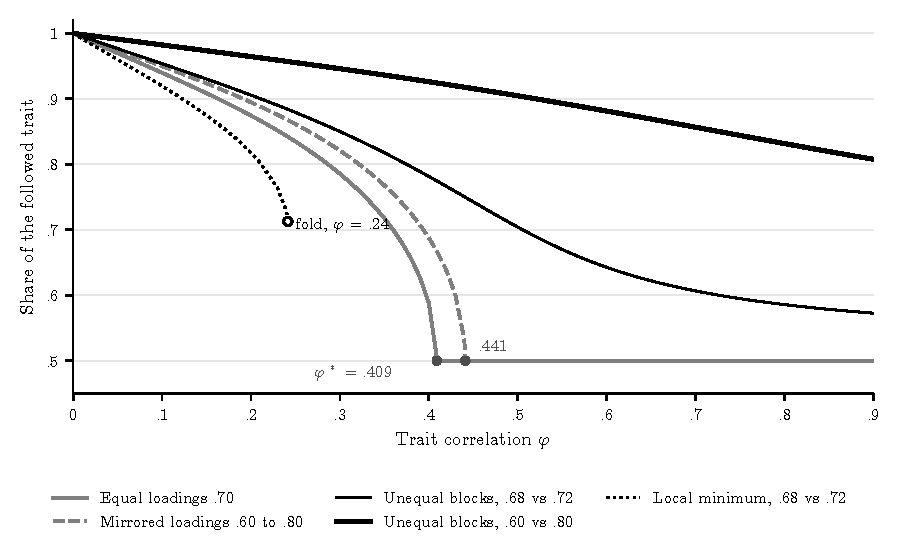
\includegraphics[width=0.85\textwidth]{fig2.pdf}
\caption{Coefficient share of the followed trait in the fitted one-factor ML model, with four items per trait. The designs have equal loadings of .70, mirrored loadings of .60, .65, .75, and .80 in each block, or different block loadings of .68 versus .72 and .60 versus .80. A share of .5 denotes an equal composite and 1 denotes one trait. For the mirrored design, the share uses block-average loadings and is approximate. The dotted curve shows the nonglobal local minimum that emphasizes the weaker block in the .68/.72 design; it ends at the fold $\varphi_f=.242$. Points on the .5 line mark where the symmetric solution loses local stability (Appendix~\ref{app:mirrored}): $\varphi^*=.409$ for equal loadings, where this is the transition, and .441 for the mirrored loadings.}
\label{fig:2}
\end{figure}

Figure~\ref{fig:2} shows that modest differences in measurement can produce substantial differences in trait representation. With loadings .68 and .72, the followed-trait share decreases smoothly from 1 at $\varphi=0$ to .77 at $\varphi=.409$, the threshold of the exchangeable design with loading .70, and to .57 at $\varphi=.9$. With loadings .6 and .8, it remains above .8 even at $\varphi=.9$. The poorer local solution can be distinguished by its discrepancy: in the .68/.72 design at $\varphi=.05$, its value is 1.25, compared with .99 at the global minimum.

Sensitivity is greatest near the exchangeable threshold. If the loadings are $\lambda-\varepsilon$ and $\lambda+\varepsilon$, Theorem~\ref{thm:cusp} in Appendix~\ref{app:unequal} shows that, for fixed interior $\lambda$ and small positive $\varepsilon$, the tilt away from equal trait representation at $\varphi^*$ is of order $\varepsilon^{1/3}$. The distance between $\varphi^*$ and the weaker solution's fold is of order $\varepsilon^{2/3}$. At $\lambda=.7$ with four items per block, a loading difference of .01 ($\varepsilon=.005$) moves the followed-trait share at $\varphi^*$ from .5 to approximately .68. The theorem concerns a local perturbation of the balanced design; its approximation is not uniform near loading zero or one.

Unequal block sizes introduce a further possibility. A longer block can dominate at low trait correlation even when its items have smaller loadings, and the favored block can change as the correlation increases. With two items loading .85 and three loading .75, the longer block is favored initially, whereas the shorter block is favored above $\varphi=.758$. Near $\varphi=1$, the comparison depends on $m_k(m_k-1)\{\lambda_k^2/(1-\lambda_k^2)\}^2$ for blocks $k=A,B$. For $.5\le\varphi<1$, these statements follow from the proof in Online Resource~3, Section~2.6. For $0<\varphi<.5$, where a worse local minimum favoring the shorter block can coexist, a computer-assisted interval-arithmetic certificate reported there (\texttt{checks/unequal\_example\_certificate.py}) shows that the minimum favoring the longer block is the unique global solution.

Such a change need not be continuous. With unequal block lengths, two local minima favoring different traits can coexist and exchange global status. At the exchange correlation they fit equally well, and the global solution jumps between them. For two items loading .90 and four loading .70, this occurs at $\varphi\approx.326$, where the share of the coefficient sum $w_A+w_B$ belonging to the shorter block's trait jumps from .10 to .92 (Online Resource~3, Section~2.6). In the example above the change is instead a smooth crossing on a unique global branch. Appendix~\ref{app:unequal} gives the exact scalar comparison and additional results for mirrored heterogeneous loadings. These extensions preserve the main implication: good approximation by one factor does not determine how that factor represents the two traits.

\subsection{Cross-Loadings and Negative Trait Correlations}
\label{sec:crossloadings}

Cross-loadings change the relation between the correlation of the generating traits and the correlation relevant to the one-factor approximation. In a design with equal, mirrored cross-loadings, this change has an exact expression. The result explains why a one-factor fit can combine information from two uncorrelated traits without contradicting the single-block solution at $\varphi=0$ in Theorem~\ref{thm:ml}. In this section, $\rho$ denotes the correlation of the generating traits, to distinguish it from the effective correlation $\varphi_{\mathrm{eff}}$ defined below.

\begin{proposition}[Equal cross-loadings]
\label{prop:crossloading}
Let each block contain $m\ge2$ items. Every item in block A has primary and secondary loadings $(\lambda_{\mathrm p},\lambda_{\mathrm s})$ on $(\theta_1,\theta_2)$, and every item in block B has loadings $(\lambda_{\mathrm s},\lambda_{\mathrm p})$. Suppose that the traits have unit variance and correlation $\rho$, and that item residuals are mutually independent, independent of the traits, and have common variance $\tau^2>0$. Define the signal variance and the between-block signal covariance
\[
\sigma_{\mathrm S}^2=\lambda_{\mathrm p}^2+\lambda_{\mathrm s}^2+2\lambda_{\mathrm p}\lambda_{\mathrm s}\rho,\qquad
\sigma_{AB}=2\lambda_{\mathrm p}\lambda_{\mathrm s}+\rho(\lambda_{\mathrm p}^2+\lambda_{\mathrm s}^2),
\]
and assume $\sigma_{\mathrm S}^2>0$. The standardized item correlation matrix has the exchangeable form of Section~\ref{sec:setup}, with $\lambda^2$ and $\varphi$ replaced by
\[
\lambda_{\mathrm{eff}}^2=\frac{\sigma_{\mathrm S}^2}{\tau^2+\sigma_{\mathrm S}^2},\qquad
\varphi_{\mathrm{eff}}=\frac{\sigma_{AB}}{\sigma_{\mathrm S}^2}
=\frac{2\lambda_{\mathrm p}\lambda_{\mathrm s}+\rho(\lambda_{\mathrm p}^2+\lambda_{\mathrm s}^2)}
{\lambda_{\mathrm p}^2+\lambda_{\mathrm s}^2+2\lambda_{\mathrm p}\lambda_{\mathrm s}\rho},
\]
where $-1\le\varphi_{\mathrm{eff}}\le1$.
\end{proposition}

\begin{proof}
Because the residuals are independent of the traits and of each other, the common signal variance of each item is $\sigma_{\mathrm S}^2$, and the signal covariance between blocks is $\sigma_{AB}$. Dividing within- and between-block covariances by the common item variance $\tau^2+\sigma_{\mathrm S}^2$ gives the stated parameters. The identities
$\sigma_{\mathrm S}^2\pm\sigma_{AB}=(1\pm\rho)(\lambda_{\mathrm p}\pm\lambda_{\mathrm s})^2$
also give $|\varphi_{\mathrm{eff}}|\le1$.
\end{proof}

For probit latent responses, $\tau^2=1$; when the loadings and residual variance are already standardized, $\lambda_{\mathrm{eff}}^2=\sigma_{\mathrm S}^2$. Negative effective correlations require only a sign change. Reversing the signs of the items in block B maps $R(\lambda,\varphi)$ to $R(\lambda,-\varphi)$ and leaves each discrepancy considered here unchanged. With $D=\diag(I_m,-I_m)$ and loadings $Dl$, the ML matrix $(D\Sigma D)^{-1}DRD=D\Sigma^{-1}RD$ has the same trace and determinant as $\Sigma^{-1}R$, and each least-squares residual $R_{ij}-l_il_j$ changes at most its sign and stays in its within-block or cross-block class. Hence, if $|\varphi_{\mathrm{eff}}|<1$, Theorem~\ref{thm:ml}, Theorem~\ref{thm:uls} and Proposition~\ref{cor:wls} apply to $(\lambda_{\mathrm{eff}},|\varphi_{\mathrm{eff}}|)$ after this reflection, using the threshold for the estimator in question. If $|\varphi_{\mathrm{eff}}|=1$, the signal is already one-dimensional. The ML classification therefore has three regimes. If $\varphi_{\mathrm{eff}}\ge\varphi^*(\lambda_{\mathrm{eff}},m)$, the best one-factor ML approximation has equal block loadings with the same sign. If $|\varphi_{\mathrm{eff}}|<\varphi^*(\lambda_{\mathrm{eff}},m)$, its loading magnitudes are unequal, and one block direction is retained at $\varphi_{\mathrm{eff}}=0$. If $\varphi_{\mathrm{eff}}\le-\varphi^*(\lambda_{\mathrm{eff}},m)$, it has equal loading magnitudes with opposite signs.

For $\lambda_{\mathrm p}>0$ and $\rho=0$, write $r=\lambda_{\mathrm s}/\lambda_{\mathrm p}$ for the secondary-to-primary slope ratio. Then $\varphi_{\mathrm{eff}}=2r/(1+r^2)$. Table~\ref{tab:2} gives the smallest nonnegative ratio for which the Gaussian one-factor ML approximation has equal block loadings. Across these designs, ratios from .08 to .22 suffice. Thus, modest cross-loadings can place uncorrelated generating traits in the equal-loading regime. This is a result for the stated latent-response populations; it does not establish the prevalence of such cross-loadings in substantive applications.

\begin{table}[t]
\centering\small
\caption{Smallest secondary-to-primary slope ratio that makes a one-factor ML fit a composite of two uncorrelated traits (probit latent responses, Gaussian analogue). Entries are the exact thresholds implied by Proposition~\ref{prop:crossloading} and Theorem~\ref{thm:ml}, rounded up to two decimals, so that each tabled ratio suffices.}
\label{tab:2}
\begin{tabular}{cccc}
\toprule
Primary probit slope & 5 items per trait & 20 items per trait & Many items \\
\midrule
.6 & .13 & .09 & .08 \\
.8 & .17 & .14 & .13 \\
1.0 & .22 & .19 & .18 \\
\bottomrule
\end{tabular}
\end{table}

The distinction matters when interpreting simulation studies that fit unidimensional IRT models to two-dimensional data. A unidimensional approximation can reflect both generating traits when items have compensatory cross-loadings, whereas exact simple structure permits a single-block solution at zero trait correlation. The Gaussian mapping provides a mechanism that can produce these different findings. It does not by itself identify the likelihood solution in every IRT design.

For example, Strachan et al. (2022) examined primary slopes from 1.2 to 1.6 and secondary slopes from .2 to .6, with a representative ratio of approximately .29. For 20 items per block, take representative logistic slopes 1.4 and .4 and divide both by 1.702 to obtain a Gaussian probit analogue. The equal-cross-loading mapping then gives the effective correlations and ML thresholds in the second and third columns of Table~\ref{tab:crossloading-illustration}. At trait correlations 0, $-.4$ and $-.8$, they place the analogue in the equal-loading, unequal-loading and bipolar regimes, respectively. At the last value, a composite constrained to have nonnegative weights cannot represent the bipolar direction. This offers a possible explanation for the instability of their nonnegative composite approximation at negative correlations.

\label{sec:crossloading-illustration}%
Heterogeneous cross-loadings produced the same qualitative regimes. We drew slopes for 20 items per trait from the ranges of Strachan et al.\ (2022), primary slopes from $U(1.2,1.6)$ and secondary slopes from $U(.2,.6)$, and divided them by 1.702 to convert the logistic metric. A one-factor model was fitted by ML to the latent-response correlation matrix, with all parameters free and 25 random starts. The best solution found was approximately balanced at $\rho=.8$, .4 and 0, favored block B at $\rho=-.4$, and formed a bipolar contrast at $\rho=-.8$ (Table~\ref{tab:crossloading-illustration}). The pattern is consistent with the effective-correlation result, but the mapping is approximate because slopes vary within blocks. These calculations concern a Gaussian latent-response analogue; they do not evaluate binary responses fitted by marginal ML. Appendix~\ref{app:binary} treats binary responses numerically.

\begin{table}[t]
\centering\small
\caption{One-factor ML fits to a Gaussian analogue of the approximate-simple-structure design of Strachan et al.\ (2022), with 20 items per trait; $\rho$ is the generating trait correlation. The effective correlation and ML threshold use the representative slopes 1.4 and .4; because slopes vary within blocks, they are approximate reference values. Slopes were drawn once (seed 22 in the supplementary code). Block loadings are the block means of the best solution found over 25 random starts, all of which reached the same objective value; signs are shown with block A positive.}
\label{tab:crossloading-illustration}
\begin{tabular}{rrrcl}
\toprule
$\rho$ & $\varphi_{\mathrm{eff}}$ & ML $\varphi^*$ & Block loadings, A / B & Regime \\
\midrule
.8 & .93 & .36 & .71 / .70 & Composite \\
.4 & .77 & .32 & .65 / .65 & Composite \\
0 & .53 & .29 & .57 / .58 & Composite \\
$-.4$ & .16 & .24 & .29 / .58 & Tilted toward B \\
$-.8$ & $-.47$ & .20 & .41 / $-.49$ & Bipolar contrast \\
\bottomrule
\end{tabular}
\end{table}


\section{Finite-Sample Behavior}
\label{sec:numerical}
\label{sec:finite-sample}

The population results imply that a one-factor model can meet a conventional fit cutoff while representing two traits, and that its loading pattern can depend on the estimator and the initial values. A finite-sample study examined both consequences; Appendix~\ref{supp:numerical} gives its details, and Appendix~\ref{app:binary} shows that the population transition also appears with binary items.

The design crossed 92 populations, four sample sizes (250, 500, 1,000 and 2,000), and three response formats (continuous, and four categories with symmetric or skewed thresholds), yielding 1,104 cells: exchangeable blocks of 4 or 8 items per trait with loading .5 or .7 (Design A), two four-item blocks with loadings .68 and .72 or .60 and .80 (Design B), and the PHQ-ADS layout of 9 and 7 items with loading .75 (Design C). Trait correlations ran from 0 to .9 in steps of .1, plus .01, .24 and .409 in Design B and further design-specific values in Designs A and C. One-factor models were fitted in lavaan (Rosseel, 2012) by ML, ULS, WLSMV and ML on ordinal scores; in Designs B and C at $N=500$ and 2,000, the ML fits also used both default item orders and 20 random starts (Appendix~\ref{supp:design}). A solution group is higher-objective when its lavaan objective exceeds that of the \emph{best solution found}, the group with the lowest observed objective, by more than $10^{-7}$; these classifications do not establish sample stationarity or global optimality.

Loading imbalance was summarized by the magnitude contrast $M=|\bar l_A|-|\bar l_B|$ between the block means of the standardized loadings and by the normalized magnitude contrast $C_{\mathrm{mag}}$ defined in Appendix~\ref{supp:design}. These quantities describe loading patterns; they are not factor-score estimates.

\subsection{Fit Indices}

Sample fit indices generally followed their population references (best-found multistart solutions, checked against the closed forms where available), although the agreement depended on the solution returned. In Designs A and C, the correlation at which half the samples met CFI $\ge.95$ or RMSEA $\le.06$ was within .03 of the population crossing point at every sample size, whereas for SRMR at $N=250$ the correlation required to pass the cutoff was up to .11 higher than the population value (Appendix~\ref{supp:fit}). For ordinal items, the population reference values of robust WLSMV CFI, TLI and RMSEA (Savalei, 2021) were within .004 of the continuous-ML population values across the evaluated populations with $\varphi\ge.7$, a numerical finding for these designs, whereas lavaan's unscaled and scaled WLSMV indices were more lenient near the cutoffs. The population agreement did not eliminate differences in small-sample cutoff-passing rates: in the PHQ-ADS layout at $N=250$ and $\varphi=.912$, robust WLSMV CFI passed less often than continuous-ML CFI, 83\% against 99\%.

\subsection{Loading Imbalance and Item Order}

The estimators differed substantially in the magnitude of sample loading imbalance (Figure~\ref{fig:4}). With four items per trait, loading .7 and $N=2{,}000$, mean $|C_{\mathrm{mag}}|$ under ML declined from .930 at $\varphi=0$ to .139 at the grid point .409 near $\varphi^*$ and .048 at .5. Under ULS, it was .317 at the ULS population threshold $1/p=.125$, and WLSMV on symmetric categories produced much less imbalance, .102 at $\varphi=0$. Thus, the population thresholds locate changes in the population solution, but sample imbalance remains positive on both sides (Appendix~\ref{supp:imbalance}).

\begin{figure}[t]
\centering
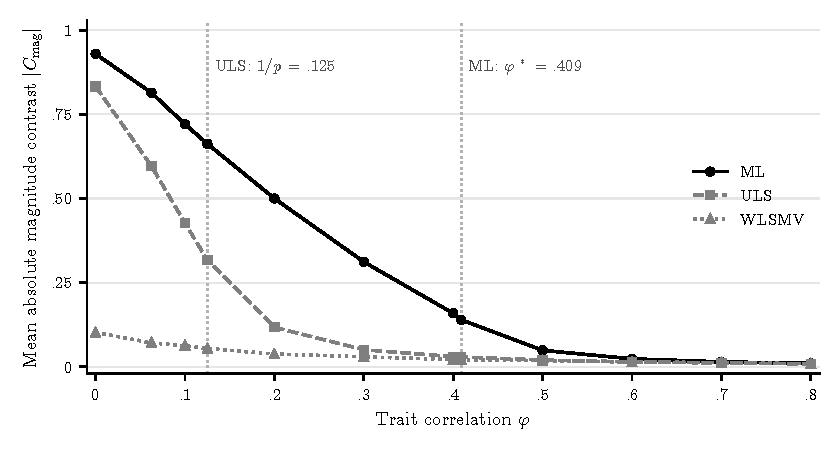
\includegraphics[width=0.85\textwidth]{fig4.pdf}
\caption{Mean absolute normalized magnitude contrast $|C_{\mathrm{mag}}|$ of one-factor fits, with 4 items per trait, loading .7 and $N=2{,}000$; WLSMV on four symmetric categories. Each point averages 1,000 continuous fits or 500 ordinal fits with valid contrasts; Monte Carlo standard errors are at most .005. The evaluated correlation $\varphi=.9$ (values below .01) is not shown. Dotted lines mark the population ML threshold $\varphi^*=.409$ and ULS threshold $1/p=.125$. Magnitudes do not encode polarity: at $\varphi=0$, opposite block signs occur in 510/1,000 ML and ULS fits and 257/500 WLSMV fits. At .0625 the counts are 15/1,000, 15/1,000 and 14/500; above .0625 they are zero on this grid.}
\label{fig:4}
\end{figure}

Item order was associated with which trait the fitted factor represented. In Design A, the two population minima below the ML threshold are mirror images, yet among default fits with $|M|>.1$ at $N=2{,}000$, the proportion with $M>.1$, favoring the first-listed block, was 86\% for continuous ML, 85\% for ML on scores, 68\% for ULS and 56\% for WLSMV (Figure~\ref{fig:5}, right). These pooled proportions are conditional on a descriptive selection, not a calibrated test. Their direction is consistent with lavaan's default starting values, which are anchored on the first-listed item.

\begin{figure}[t]
\centering
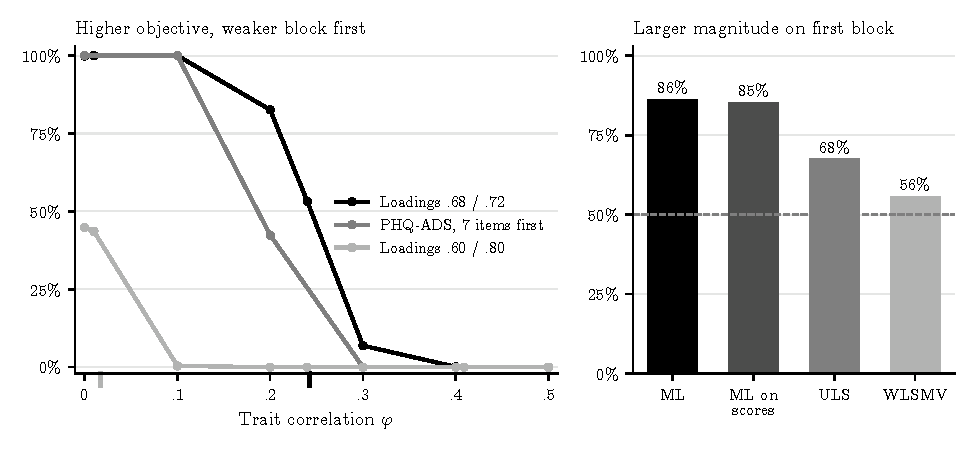
\includegraphics[width=\textwidth]{fig5.pdf}
\caption{Item order and lavaan's default start, $N=2{,}000$. Left: share of continuous ML fits assigned to a higher-objective solution group that follows the weaker block when that block is listed first. Each point uses 1,000 archived replications. Ticks mark the two Design B population folds. Right: pooled share of magnitude-selected fits ($|M|>.1$) with $M>.1$ in the exchangeable design, over all four conditions and their complete correlation grids. ML and ULS use continuous items; ML on scores and WLSMV use symmetric four-category items. Selected/attempted fits are 28,719/53,000 (ML), 13,501/26,500 (ML on scores), 18,344/53,000 (ULS) and 4,746/26,500 (WLSMV); the pooled shares are dominated by low-correlation cells, where $|M|>.1$ is common. The dashed line is the 50\% reference. Solution groups do not certify sample minima.}
\label{fig:5}
\end{figure}

When the blocks differed, item order could also lower the fit reported from the default start (Figure~\ref{fig:5}, left; Table~\ref{tab:4}). With the weaker block listed first, continuous ML returned a higher-objective group favoring that block in 94 to 100\% of samples at $\varphi\le.1$ and $N=500$ and 2,000, both with loadings .68 and .72 and in the PHQ-ADS layout with the 7-item block first. Listing the weaker block last produced no weaker-block flags in the 234 archived cell--analysis combinations, although 761 of the 156,000 multistart replications retained a higher-objective group under that order. In the PHQ-ADS layout with depression items listed first, the default-order weaker-block flag was absent in these simulations; that result does not establish which solution was obtained in the published trials.

\begin{table}[t]
\centering\small
\caption{Continuous ML in Designs B and C: population reference CFI, mean sample CFI, and the frequency of higher-objective weaker-block solutions. Default starts use design order: the weaker block first in Design B and the stronger block first in Design C. Each sample entry uses 1,000 paired replications; Monte Carlo standard errors of the percentages are at most 1.6 percentage points. The best solution found is the retained solution group with the lowest observed objective. Its CFI is reconstructed using the estimated baseline noncentrality; all 18,000 pairs satisfy the inversion domain. Population entries are best-found numerical reference values from multistart fitting; no closed form applies to these designs.}
\label{tab:4}
\setlength{\tabcolsep}{3pt}
\begin{tabularx}{\textwidth}{@{}>{\raggedright\arraybackslash}p{3.7cm}c*{5}{>{\centering\arraybackslash}X}>{\centering\arraybackslash}p{2.1cm}@{}}
\toprule
Design and order & $\varphi$ & Population CFI & Default start, $N = 500$ & Default start, $N = 2{,}000$ & Best found, $N = 500$ & Best found, $N = 2{,}000$ & Higher-objective weaker group, $N = 500$ / 2,000 \\
\midrule
.68 and .72, weaker first & 0 & .558 & .443 & .442 & .561 & .559 & 95\% / 99.9\% \\
.68 and .72, weaker first & .1 & .567 & .460 & .454 & .568 & .567 & 94\% / 100\% \\
.68 and .72, weaker first & .2 & .591 & .538 & .513 & .595 & .592 & 65\% / 83\% \\
.68 and .72, weaker first & .24 & .606 & .571 & .563 & .607 & .606 & 49\% / 53\% \\
.68 and .72, weaker first & .3 & .632 & .618 & .630 & .632 & .633 & 26\% / 7\% \\
.60 and .80, weaker first & 0 & .767 & .630 & .533 & .767 & .766 & 28\% / 45\% \\
.60 and .80, weaker first & .1 & .771 & .731 & .768 & .768 & .770 & 8\% / 0.4\% \\
PHQ-ADS layout, stronger first & 0 & .585 & .585 & .585 & .585 & .585 & 0\% / 0\% \\
PHQ-ADS layout, stronger first & .1 & .590 & .590 & .590 & .590 & .590 & 0\% / 0\% \\
\bottomrule
\end{tabularx}
\end{table}

Higher-objective weaker-block groups also occurred above the population fold (Table~\ref{tab:4}, $\varphi=.3$) and have no sample stationarity certificate. In all 156,000 archived multistart replications, at least one default-order group was within $10^{-7}$ in lavaan objective of the best group found with the additional random starts, so checking both item orders was useful in this study; this result concerns the evaluated designs and retained groups and does not guarantee global optimality.

\section{An Illustration Based on Published PHQ-ADS Results}
\label{sec:phq}

The PHQ-ADS illustrates why the fit of a merged model and the interpretation of its factor require separate assessment. Kroenke et al.\ (2016) fitted one-factor, two-factor and bifactor models to its 9 depression and 7 anxiety items in three trials of patients with chronic pain or cancer: SCOPE ($n=250$), ESCAPE ($n=241$) and INCPAD ($n=405$). The reported two-factor correlations were .912, .865 and .653, respectively. We use these correlations, the published two-factor loadings and the block lengths in a population calculation, with a common loading as a sensitivity analysis, to show how the theoretical results can inform interpretation.

The calculation assumes an exactly fitting two-factor population with the two-factor loadings reported by Kroenke et al.\ (2016, Supplemental Digital Content, Table S3). The sensitivity calculation replaces these loadings by a common loading between .70 and .80. Neither calculation is a reconstruction of the trial-specific fits. There is also an estimator difference: the published analysis treated the responses as ordered categorical in Mplus with a logistic link, whereas the population calculation applies normal-theory ML and treats the published standardized loadings as latent-response loadings. Categorical estimation can change the fit indices (Lubbe, 2023). Finally, the reported two-factor RMSEA exceeded .06 in all three trials. The population calculation therefore isolates the discrepancy due to merging the two traits under the stated assumptions; it does not allocate the observed misfit between omitted dimensionality and other sources.

\begin{table}[t]
\centering\small
\caption{Published PHQ-ADS fit indices and the population one-factor approximation. Reported values are from Kroenke et al.\ (2016), their Table 5. Population values assume an exact two-factor model with 9 depression and 7 anxiety items and the published trait correlation. Its loadings are either the published two-factor loadings (Kroenke et al., 2016, Supplemental Digital Content, Table S3) or, as a sensitivity analysis, a common loading from .70 to .80. The one-factor approximation is fitted by normal-theory ML. With the published loadings the solution is the best found by multistart numerical minimization; with a common loading it follows from the scalar classification of Appendix~\ref{app:unequal-scalar}. The last column reports the depression coefficient share in that population approximation, not the share in the published trial fit or a factor score.}
\label{tab:5}
\setlength{\tabcolsep}{4pt}
\begin{tabularx}{\textwidth}{lLLLLLLL}
\toprule
Trial & Trait correlation & Reported 1-factor RMSEA, CFI & Reported 2-factor RMSEA, CFI & Loadings & Population RMSEA & Population CFI & Depression share of the fitted factor \\
\midrule
SCOPE & .912 & .091, .956 & .085, .962 & Published & .058 & .967 & .46 \\
 & & & & Common & .037 to .060 & .969 to .981 & .58 to .59 \\
\addlinespace
ESCAPE & .865 & .083, .954 & .071, .967 & Published & .065 & .951 & .53 \\
 & & & & Common & .052 to .083 & .941 to .962 & .59 to .60 \\
\addlinespace
INCPAD & .653 & .130, .862 & .085, .941 & Published & .122 & .803 & .33 \\
 & & & & Common & .103 to .149 & .796 to .840 & .64 to .70 \\
\bottomrule
\end{tabularx}
\end{table}

The illustration shows three substantively different patterns (Table~\ref{tab:5}). At INCPAD's correlation of approximately .65, the one-factor population with the published loadings has RMSEA .122 and CFI .803, and the common-loading range gives RMSEA from .10 to .15 and CFI from .80 to .84. These values are of similar magnitude to the reported .130 and .862 and show that merging traits can itself produce substantial misfit in this range. At ESCAPE's correlation of .865, the published loadings give CFI $=.951$ but RMSEA $=.065$, the same kind of disagreement between conventional cutoffs that ESCAPE reported; a common loading near .75 gives CFI $=.953$ and RMSEA $=.065$. At SCOPE's correlation of .912, population RMSEA is .058 with the published loadings and ranges from .037 to .060 with a common loading (.0602 at loading .80, marginally above the cutoff), and CFI exceeds .96 in both calculations. The reported RMSEA is .091 for one factor and .085 for two factors, so failure of the one-factor RMSEA cutoff alone cannot attribute the discrepancy to merging depression and anxiety.

The disagreement between CFI and RMSEA follows from their different denominators. For this 16-item one-factor model, RMSEA divides the discrepancy by 104 degrees of freedom and meets .06 only when $F_{\min}\le.06^2\times104\approx.374$. CFI divides the same discrepancy by the independence-model discrepancy, which is 8.9 at ESCAPE's correlation with the published ESCAPE loadings. With these loadings, CFI reaches .95 from a trait correlation of approximately .864 and RMSEA reaches .06 from approximately .878, so ESCAPE's correlation of .865 lies just inside the interval in which the two cutoffs disagree. In the common-loading sensitivity calculation at $\varphi=.865$, the independence-model discrepancy is 7.3 for a common loading of .70, 9.4 for .75, and 12.0 for .80. With loading .70, the one-factor model meets both cutoffs from a correlation of approximately .84. With loading .75, the CFI threshold is .86 and the RMSEA threshold is .88; with loading .80, the disagreement interval extends from .88 to .912, so SCOPE's correlation lies at its upper edge. Thus, the interval widens with the loadings in this sensitivity calculation.

Which trait the fitted factor favors depends on the block lengths and the loadings together. With a common loading, the longer depression block carries more multi-information and receives a coefficient share of .58 to .59 at SCOPE's correlation and .64 to .70 at INCPAD's. The corresponding depression shares in regression or Bartlett scores are .57 to .58 and .63 to .68, compared with $9/16=.56$ in the unit-weighted sum score. With the published two-factor loadings, depression receives the larger coefficient share only in ESCAPE. In all three trials the anxiety items have higher two-factor loadings on average than the depression items, with block means of .72 and .80 in SCOPE, .71 and .75 in ESCAPE, and .66 and .75 in INCPAD, and the population one-factor approximation gives depression a coefficient share of .46, .53 and .33. When the blocks differ in length, the higher loadings alone do not determine which trait the factor favors (Section~\ref{sec:unequal}). The anxiety block has the larger total correlation in SCOPE (2.43 against 2.39) and INCPAD (2.02 against 1.70), whereas in ESCAPE the smaller loading difference leaves the larger total correlation with the longer depression block (2.13 against 1.81). With one summary loading per block, the comparison of $m_k(m_k-1)\{\lambda_k^2/(1-\lambda_k^2)\}^2$ that applies as $\varphi$ approaches 1 orders the blocks in the same way, and in these calculations the favored block is the same at every trait correlation.

The one-factor loadings implied by the published two-factor solutions agree closely with the published one-factor loadings: across the 16 items their correlations are 1.000, .999 and .961. With the published two-factor loadings as reference, the published one-factor loadings give depression coefficient shares of .46, .51 and .44. At INCPAD's correlation the regression factor score correlates .81 with depression and .94 with anxiety, whereas the unit-weighted sum correlates .89 and .87. The factor share and score share are distinct quantities, and the factor score and the sum score represent the two traits differently.

These results establish the behavior of the specified population model, not the composition of the published PHQ-ADS scores. The published loadings are estimates from a categorical model, and the reported samples add sampling uncertainty; for example, ESCAPE had $n=241$ and sample RMSEA .083 with 104 degrees of freedom. The finite-sample study provides relevant design-based context, but neither that study nor this illustration removes the estimator difference or the misspecification of the published two-factor model.

\section{Discussion}
\label{sec:discussion}

The best one-factor approximation to two correlated traits has a systematic, design-dependent interpretation. With equal item blocks, ML gives an equal composite above a known correlation threshold and favors one trait below it; when the blocks differ, the global solution can favor one trait throughout the correlation range, and an inferior local minimum can favor the other. With unequal block lengths, the favored trait can also switch abruptly at a correlation where two different solutions fit equally well. These changes in representation are accompanied by exact changes in population fit, so the formulas make it possible to examine both what the fitted factor represents and what a fit criterion can distinguish for a specified measurement design.

\subsection{Interpreting One-Factor Fit}

The cutoff boundaries in Table~\ref{tab:1} quantify the limits of an inference from acceptable fit to unidimensionality: each gives the trait correlation from which a conventional cutoff is met although two traits generate the data. Every CFI boundary in Table~\ref{tab:1} lies above the ML transition, so in these equal-block designs the approximation meeting the CFI cutoff is a composite. This need not hold for every index: with loading .50 and four items, the SRMR cutoff is met at every correlation, including the tilted regime. A tilted solution and an acceptable fit are therefore separate findings, although unequal blocks can make trait representation unbalanced even at high correlations. Neither the fit index nor the number of fitted factors alone specifies the contribution of each trait, and a fit index is not a measure of the substantive importance of a trait.

Rather than a universal replacement cutoff, the analysis supplies a benchmark conditional on the proposed item structure, which can be reported alongside the observed indices and examined over plausible loading values. Such a calculation makes the evidential limits of a merged-factor comparison explicit, particularly when absolute fit of the merged model is treated as evidence against discriminant validity (R\"onkk\"o \& Cho, 2022). It complements simulation-based dynamic fit indices, whose one-factor implementation considers residual correlations as the source of misspecification (McNeish \& Wolf, 2023), and the simulation-cum-ROC approach of Groskurth et al.\ (2025), which permits a two-factor alternative to a one-factor model and selects cutoffs from simulated classification performance. The boundaries derived here identify the population trait correlations at which a fixed cutoff is met; they do not calibrate finite-sample type I and type II error rates.

Interpretation also requires the loading pattern, the intended score and the estimator. For a specified two-trait generating model, the fitted loadings determine the trait contributions only together with the generating loadings; raw one-factor loadings alone do not identify the factor's trait composition. The composition of an estimated factor must also be distinguished from that of a score computed from the items: regression and Bartlett factor scores have the same relative trait contributions in the setting considered here, but these generally differ from those of the fitted factor and the unit-weighted sum. Reporting one score therefore requires an interpretation of that score's weights as well as an assessment of model fit. ML, unweighted least squares, and principal components can represent different directions for the same population correlation matrix, so the estimation criterion matters beyond standard errors and goodness-of-fit corrections. Likewise, the close agreement of lavaan's robust categorical indices (Savalei, 2021) with the continuous-ML references near the cutoffs is a numerical result for the studied designs and does not identify the categorical fitted factor with the ML fitted factor.

\subsection{Computation and Reporting}

In the finite-sample study, item order, an arbitrary feature of the input, was associated with which trait the default-start solution favored and, when the blocks differed, with whether that solution had a higher objective and favored the weaker block, consistent with lavaan's default starting values, which are anchored on the first-listed item (Section~\ref{sec:numerical}). For a one-factor model fitted to known item blocks, a useful check is therefore to compare the solutions obtained with each block listed first and with additional starting values, retaining the discrepancy and loading pattern of each distinct solution. The archived multistart results support this check for the studied designs (Section~\ref{sec:numerical}) but do not prove that two orders are sufficient in general. Moreover, agreement in objective and reported convergence do not by themselves establish stationarity or a local minimum: the population refits showed that equal starting covariances could lead to different trajectories under different identifications, including a symmetric saddle. When competing solutions affect interpretation, objective comparisons should be accompanied by checks of the relevant first- and second-order conditions.

The boundary criterion of Proposition~\ref{prop:boundary} (Appendix~\ref{app:heywood-proof}) has a separate use. For a one-factor ML model with nonnegative uniquenesses, it gives a necessary condition for a solution with one zero uniqueness to be a local minimum. In the two-trait population it excludes such minima except at the stated two-item, zero-correlation endpoint; more generally, it can rule out a reported zero-uniqueness solution when releasing that uniqueness decreases the discrepancy. The result does not classify unconstrained negative uniqueness estimates or solutions obtained by other estimators.

The accompanying R package \texttt{undeRfactor} (version 0.2.0, \url{https://github.com/atomashevic/undeRfactor}) implements the population calculations, the ML, ULS and WLSMV transition thresholds (\texttt{phi\_star()}), the ML cutoff boundaries (\texttt{blind\_spot()}), all stationary points of designs with one loading per block from the quartic of Appendix~\ref{app:unequal-scalar} (\texttt{block\_solutions()}), the candidate-solution search, the coefficient and score shares, the one-factor solution implied by an estimated two-factor model (\texttt{predict\_one\_factor()}) and the item-order check. Closed forms and the quartic are used where available; elsewhere, the package reports the distinct candidates found and does not certify global optimality. Coefficient shares describe covariance matching rather than explained variance; signed shares depend on trait orientation and are undefined when the coefficients sum to zero, and nonzero reference block means and $|\varphi|<1$ are required for identification.

\subsection{Scope and Further Work}

The exact results concern a structured two-trait population. The exchangeable case permits a closed global solution, and constant loadings within unequal blocks permit an exact reduction to a quartic equation. For unequal block lengths, this reduction gives a selection rule but not a closed partition of the full design space, and the global solution need not vary continuously with the trait correlation (Section~\ref{sec:unequal}). For loadings that vary within blocks, the general information-loss bound (Appendix~\ref{app:ceiling}) and numerical examples provide partial results. Independent residuals are part of the generating model, and more than two traits are outside the present analysis. These restrictions isolate a mechanism that is difficult to identify from numerical optimization alone, but they also limit direct application of the formulas to heterogeneous instruments. Matching lower bounds for variable loadings, a full classification of competing minima with unequal block lengths, and extensions to more than two traits are therefore priorities for further analytic work.

The population and finite-sample conclusions have different scopes: the normal-theory ML theorems concern the population objective, whereas the simulation study covers sample sizes from 250 to 2,000 and the specified continuous and ordinal designs. The study does not establish performance for smaller samples, nonnormal continuous responses, or every set of ordinal thresholds; in particular, different item thresholds generally remove the two-weight structure used in the weighted least-squares result. Archived solution groups identify alternatives found by the specified starts but do not certify sample stationarity or global optimality. The power summaries use conventional noncentral-$\chi^2$ approximations; their finite-sample accuracy, especially near the transition and at nonregular endpoints, was not assessed.

The cross-loading and application results require corresponding qualifications. Equal cross-loadings yield an exact transformation of the latent-response covariance into the two-block form. The Gaussian analogue of the Strachan et al.\ (2022) design suggests a mechanism for their reported instability at negative correlations but is not a replication of binary marginal-ML estimation, and the binary calculations (Appendix~\ref{app:binary}) provide numerical evidence rather than a general theorem for IRT models. Likewise, the PHQ-ADS illustration applies normal-theory ML to the published two-factor loadings, which were estimated from ordered categorical responses with a logistic link, and uses a common-loading range of .70 to .80 as a sensitivity analysis. It is therefore not an exact reanalysis of the original categorical responses and cannot by itself validate the total score.

The exchangeable two-trait population also admits a bifactor representation with general loadings $\lambda\sqrt{\varphi}$ and specific loadings $\lambda\sqrt{1-\varphi}$, whose explained common variance is therefore $\varphi$, linking the present thresholds to an index used to assess essential unidimensionality (Reise et al., 2013; Rodriguez et al., 2016). The present results already show why one-factor fit should be reported together with the design, the estimator, and the trait representation of the solution that was obtained.

% The named preprint carries the full Declaration of AI Use (declarations.tex).
\ifdefined\preprint\else
\paragraph{Use of AI tools.}
The mathematical proofs reported in this article and in Online Resources 1--3 were developed with the assistance of the large language model ChatGPT 6 Pro (OpenAI). The large language model Claude Opus 5.5 (Anthropic) assisted with writing the code and with preparing and editing the manuscript.
\fi

\ifdefined\preprint% Declarations shared by the cover page (cover_page.tex) and the named preprint
% (main.tex built with \def\preprint{}). Edit them here only.

\section*{Data Availability}
The code, archived simulation summaries, portable evidence files and the complete proofs (Online Resources 1--3) supporting this article are available at \url{https://github.com/atomashevic/one-factor-two-traits} and archived at Zenodo (\url{https://doi.org/10.5281/zenodo.23670526}). The R package \texttt{undeRfactor}, version 0.2.0, which implements the population calculations, is available at \url{https://github.com/atomashevic/undeRfactor} and archived at Zenodo (\url{https://doi.org/10.5281/zenodo.23668208}). The raw output of the 2.3 million model fits in the simulation study is not included in the repository and is available from the author on request. No new empirical data were collected for this article; the PHQ-ADS illustration is based on published results.

\section*{Financial Support}
This research received no specific grant funding from any funding agency, commercial or not-for-profit sectors.

\section*{Competing Interests}
The author declares none.

\section*{Declaration of AI Use}
The mathematical proofs reported in this article and in Online Resources 1--3 were developed with the assistance of the large language model ChatGPT 6 Pro (OpenAI), accessed through the ChatGPT web interface. The large language model Claude Opus 5.5 (Anthropic), accessed through Claude Code, assisted with writing the code and with preparing and editing the manuscript. The author reviewed this content and takes responsibility for it.
% The journal's AI policy asks for the name and version of each tool, the dates of use as far as
% reasonably possible, how others can access the tool and how it was used. The author chose not
% to give dates of use (26 October 2026). The anonymised
% manuscript carries the same statement without access details (end of the Discussion); keep
% the two consistent.
\fi
\clearpage
\section*{References}
\begingroup\small\setlength{\parindent}{-1.5em}\setlength{\leftskip}{1.5em}
Ackerman, T. A. (1989). Unidimensional IRT calibration of compensatory and noncompensatory multidimensional items. \textit{Applied Psychological Measurement, 13}(2), 113--127. \url{https://doi.org/10.1177/014662168901300201}

Akaike, H. (1987). Factor analysis and AIC. \textit{Psychometrika, 52}(3), 317--332. \url{https://doi.org/10.1007/BF02294359}

Ansley, T. N., \& Forsyth, R. A. (1985). An examination of the characteristics of unidimensional IRT parameter estimates derived from two-dimensional data. \textit{Applied Psychological Measurement, 9}(1), 37--48. \url{https://doi.org/10.1177/014662168500900104}

Baik, J., Ben Arous, G., \& Péché, S. (2005). Phase transition of the largest eigenvalue for nonnull complex sample covariance matrices. \textit{Annals of Probability, 33}(5), 1643--1697. \url{https://doi.org/10.1214/009117905000000233}

Chun, S. Y., \& Shapiro, A. (2009). Normal versus noncentral chi-square asymptotics of misspecified models. \textit{Multivariate Behavioral Research, 44}(6), 803--827. \url{https://doi.org/10.1080/00273170903352186}

Cudeck, R., \& Browne, M. W. (1992). Constructing a covariance matrix that yields a specified minimizer and a specified minimum discrepancy function value. \textit{Psychometrika, 57}(3), 357--369. \url{https://doi.org/10.1007/BF02295424}

Dijkstra, T. K. (1990). Some properties of estimated scale invariant covariance structures. \textit{Psychometrika, 55}(2), 327--336. \url{https://doi.org/10.1007/BF02295290}

Fukasaku, R., Hirose, K., Kabata, Y., \& Teramoto, K. (2025). Algebraic approach to maximum likelihood factor analysis. \textit{Psychometrika, 90}(5), 1732--1764. \url{https://doi.org/10.1017/psy.2025.10047}

Golubitsky, M., \& Schaeffer, D. G. (1985). \textit{Singularities and groups in bifurcation theory} (Vol.~1). Springer. \url{https://doi.org/10.1007/978-1-4612-5034-0}

Groskurth, K., Bhaktha, N., \& Lechner, C. M. (2025). The simulation-cum-ROC approach: A new approach to generate tailored cutoffs for fit indices through simulation and ROC analysis. \textit{Behavior Research Methods, 57}(5), Article 135. \url{https://doi.org/10.3758/s13428-025-02638-x}

Groskurth, K., Bluemke, M., \& Lechner, C. M. (2024). Why we need to abandon fixed cutoffs for goodness-of-fit indices: An extensive simulation and possible solutions. \textit{Behavior Research Methods, 56}(4), 3891--3914. \url{https://doi.org/10.3758/s13428-023-02193-3}

Hancock, G. R., \& Mueller, R. O. (2011). The reliability paradox in assessing structural relations within covariance structure models. \textit{Educational and Psychological Measurement, 71}(2), 306--324. \url{https://doi.org/10.1177/0013164410384856}

Heene, M., Hilbert, S., Draxler, C., Ziegler, M., \& Bühner, M. (2011). Masking misfit in confirmatory factor analysis by increasing unique variances. \textit{Psychological Methods, 16}(3), 319--336. \url{https://doi.org/10.1037/a0024917}

Horn, R. A., \& Johnson, C. R. (2013). \textit{Matrix analysis} (2nd ed.). Cambridge University Press.

Hu, L., \& Bentler, P. M. (1999). Cutoff criteria for fit indexes in covariance structure analysis. \textit{Structural Equation Modeling, 6}(1), 1--55. \url{https://doi.org/10.1080/10705519909540118}

Kenny, D. A., \& McCoach, D. B. (2003). Effect of the number of variables on measures of fit in structural equation modeling. \textit{Structural Equation Modeling, 10}(3), 333--351. \url{https://doi.org/10.1207/S15328007SEM1003_1}

Kroenke, K., Wu, J., Yu, Z., Bair, M. J., Kean, J., Stump, T., \& Monahan, P. O. (2016). Patient Health Questionnaire Anxiety and Depression Scale: Initial validation in three clinical trials. \textit{Psychosomatic Medicine, 78}(6), 716--727. \url{https://doi.org/10.1097/PSY.0000000000000322}

Lai, K., \& Green, S. B. (2016). The problem with having two watches: Assessment of fit when RMSEA and CFI disagree. \textit{Multivariate Behavioral Research, 51}(2--3), 220--239. \url{https://doi.org/10.1080/00273171.2015.1134306}

Lawley, D. N. (1956). Tests of significance for the latent roots of covariance and correlation matrices. \textit{Biometrika, 43}(1--2), 128--136. \url{https://doi.org/10.1093/biomet/43.1-2.128}

Lubbe, D. (2023). Advantages of using unweighted approximation error measures for model fit assessment. \textit{Psychometrika, 88}(2), 413--433. \url{https://doi.org/10.1007/s11336-023-09909-6}

McNeish, D., An, J., \& Hancock, G. R. (2018). The thorny relation between measurement quality and fit index cutoffs in latent variable models. \textit{Journal of Personality Assessment, 100}(1), 43--52. \url{https://doi.org/10.1080/00223891.2017.1281286}

McNeish, D., \& Wolf, M. G. (2023). Dynamic fit index cutoffs for one-factor models. \textit{Behavior Research Methods, 55}(3), 1157--1174. \url{https://doi.org/10.3758/s13428-022-01847-y}

Moshagen, M., \& Auerswald, M. (2018). On congruence and incongruence of measures of fit in structural equation modeling. \textit{Psychological Methods, 23}(2), 318--336. \url{https://doi.org/10.1037/met0000122}

Paul, D. (2007). Asymptotics of sample eigenstructure for a large dimensional spiked covariance model. \textit{Statistica Sinica, 17}(4), 1617--1642. \url{https://www3.stat.sinica.edu.tw/statistica/oldpdf/A17n418.pdf}

R Core Team. (2025). \textit{R: A language and environment for statistical computing} (Version 4.5.1) [Computer software]. R Foundation for Statistical Computing. \url{https://www.R-project.org/}

Reckase, M. D. (1979). Unifactor latent trait models applied to multifactor tests: Results and implications. \textit{Journal of Educational Statistics, 4}(3), 207--230. \url{https://doi.org/10.3102/10769986004003207}

Reise, S. P., Scheines, R., Widaman, K. F., \& Haviland, M. G. (2013). Multidimensionality and structural coefficient bias in structural equation modeling: A bifactor perspective. \textit{Educational and Psychological Measurement, 73}(1), 5--26. \url{https://doi.org/10.1177/0013164412449831}

Rodriguez, A., Reise, S. P., \& Haviland, M. G. (2016). Evaluating bifactor models: Calculating and interpreting statistical indices. \textit{Psychological Methods, 21}(2), 137--150. \url{https://doi.org/10.1037/met0000045}

Rönkkö, M., \& Cho, E. (2022). An updated guideline for assessing discriminant validity. \textit{Organizational Research Methods, 25}(1), 6--47. \url{https://doi.org/10.1177/1094428120968614}

Rosseel, Y. (2012). lavaan: An R package for structural equation modeling. \textit{Journal of Statistical Software, 48}(2), 1--36. \url{https://doi.org/10.18637/jss.v048.i02}

Savalei, V. (2021). Improving fit indices in structural equation modeling with categorical data. \textit{Multivariate Behavioral Research, 56}(3), 390--407. \url{https://doi.org/10.1080/00273171.2020.1717922}

Shi, D., Lee, T., \& Maydeu-Olivares, A. (2019). Understanding the model size effect on SEM fit indices. \textit{Educational and Psychological Measurement, 79}(2), 310--334. \url{https://doi.org/10.1177/0013164418783530}

Strachan, T., Cho, U. H., Ackerman, T., Chen, S., de la Torre, J., \& Ip, E. H. (2022). Evaluation of the linear composite conjecture for unidimensional IRT scale for multidimensional responses. \textit{Applied Psychological Measurement, 46}(5), 347--360. \url{https://doi.org/10.1177/01466216221084218}

Tipping, M. E., \& Bishop, C. M. (1999). Probabilistic principal component analysis. \textit{Journal of the Royal Statistical Society: Series B (Statistical Methodology), 61}(3), 611--622. \url{https://doi.org/10.1111/1467-9868.00196}

Watanabe, S. (1960). Information theoretical analysis of multivariate correlation. \textit{IBM Journal of Research and Development, 4}(1), 66--82. \url{https://doi.org/10.1147/rd.41.0066}

\endgroup

\clearpage
\appendix
\section{Main Steps in the Proof of Theorem~\ref{thm:ml}}
\label{app:ml}

This appendix presents the reductions that give the unrestricted ML solution. The complete proof, including the separate endpoint argument and all equality cases, is given in Online Resource~1. We retain the notation of Section~\ref{sec:setup}.

\subsection{Existence and Interior Score Equations}

Let $\mu_1,\ldots,\mu_p$ be the eigenvalues of $R^{1/2}\Sigma^{-1}R^{1/2}$. Then
\[
F(\Sigma)=\sum_{i=1}^p g(\mu_i),\qquad g(t)=t-\log t-1.
\]
Because $g$ is nonnegative and tends to infinity at both ends of $(0,\infty)$, a sublevel set $\{F\le c\}$ bounds $\Sigma$ above and away from singularity. The one-factor model is closed relative to the positive-definite cone: along a convergent sequence of feasible covariances, $l_i^2\le\Sigma_{ii}$ and $0\le\psi_i\le\Sigma_{ii}$ bound the parameters and give a convergent feasible subsequence. Since the identity matrix is feasible, a minimizing sequence lies in a nonempty compact sublevel set. The discrepancy therefore attains its minimum.

For fixed $\Psi\succ0$, write $B=\Psi^{-1/2}R\Psi^{-1/2}$, the population matrix whitened by the uniquenesses, and $v=\Psi^{-1/2}l$. The rank-one inverse and determinant identities give
\[
F=\tr B-\log\det B-p
-\frac{v^{\top}Bv}{1+v^{\top}v}+\log(1+v^{\top}v).
\]
At fixed $v^{\top}v$, the minimizing direction is a leading eigenvector of $B$. If the ordered eigenvalues of $B$ are $\zeta_1\ge\cdots\ge\zeta_p$, minimization over the norm gives $v^{\top}v=\max(\zeta_1-1,0)$ and concentrated discrepancy
\[
\min_l F=
\begin{cases}
\displaystyle\sum_{j=2}^p g(\zeta_j),&\zeta_1>1,\\[2pt]
\displaystyle\sum_{j=1}^p g(\zeta_j),&\zeta_1\le1.
\end{cases}
\]
At a nonzero local minimum over the loading vector, $v$ is an eigenvector of $B$ (stationarity at fixed norm) and must be a leading one, since rotation toward an eigenvector with a larger eigenvalue lowers the discrepancy.

At an interior stationary point, put $u=\Psi^{-1}l$ and $\gamma=l^{\top}u$. Differentiation with respect to the loadings and uniquenesses gives
\begin{equation}
Ru=(1+\gamma)l,
\qquad \psi_i=1-l_i^2,
\label{eq:ml-scores}
\end{equation}
so the fitted variances equal the population variances. An equivalent row equation is
\begin{equation}
\sum_{j\ne i}u_j(R_{ij}-l_il_j)=0.
\label{eq:ml-row-score}
\end{equation}
When $\varphi>0$, $B$ has strictly positive entries. Perron's theorem implies that its leading eigenvalue is simple and has a strictly positive eigenvector (Horn \& Johnson, 2013, Ch.~8). The zero-loading stationary point is not a minimum because the leading eigenvalue of $R$ exceeds one. Thus every interior local minimum has strictly positive loadings after a common sign change.

\subsection{Boundary Exclusion and the Reduction to Two Loadings}

A positive-definite one-factor covariance can have at most one zero uniqueness. Proposition~\ref{prop:boundary} characterizes the only stationary candidate on each such boundary face and gives its inward derivative. For the present population that derivative is strictly negative except when $m=2$ and $\varphi=0$. Hence all local minima at positive trait correlation are interior.

For an item in A, equation~\eqref{eq:ml-scores} can be written
\[
(1+\gamma)l_i-a\frac{l_i}{1-l_i^2}=C_A,
\]
with the same $C_A$ throughout the block. The left side is strictly concave on $(0,1)$, so there are at most two loading values within a block. If those values are $x<y$, elimination of $C_A$ gives
\[
\gamma_{\mathrm{rest}}(1-x^2)(1-y^2)=(1+xy)(xy-L),
\]
where $i$ and $j$ are items with loadings $x$ and $y$, and $\gamma_{\mathrm{rest}}=\sum_{k\ne i,j}l_k^2/\psi_k>0$ is the contribution of the other items to $\gamma$. Therefore $xy>L$.

The row equation for an item loading $y$ now has negative within-block residuals. It must have a positive cross-block residual, so $yz<L\varphi$ for the smallest loading $z$ in B. Since $xy>L$ gives $y>\lambda$, we have $z<L\varphi/y<\lambda$. The row equation for $z$ then has positive cross-block residuals, so some within-block residual $L-zw$ in that row is negative. Hence B contains a second loading $w>L/z>\lambda>z$, with $zw>L$. Applying the same argument to $w$ gives $wx<L\varphi$. This is impossible, because
\[
(xy)(zw)>L^2,
\qquad
(yz)(wx)<L^2\varphi^2<L^2,
\]
whereas the left sides are equal. Each local minimum at $\varphi>0$ must therefore have constant loadings within each block. Appendix~\ref{app:unequal-reduction} gives the corresponding argument for unequal blocks.

\subsection{The Global Scalar Comparison}

For block-uniform uniquenesses, let $\Psi=\diag(\psi_AI_m,\psi_BI_m)$ and write $\psi_A=e^{s+d}$ and $\psi_B=e^{s-d}$. Before multiplication by $e^{-s}$, the two block-mean eigenvalues are
\[
T_\pm(d)=b\cosh d\pm\sqrt{b^2\sinh^2d+h^2}.
\]
The leading eigenvalue is $T_+$; the sum of the remaining $\nu $ eigenvalues is $Q(d)=2na\cosh d+T_-(d)$. Minimization over the common scale gives $e^s=Q(d)/\nu $ and leaves
\[
\mathcal H(d)=\nu \log\frac{Q(d)}\nu -2n\log a-\log T_-(d).
\]
The optimal scale belongs to the active-factor region because $Q<\nu T_+$. In the diagonal-model region, where the leading whitened eigenvalue is at most one, the discrepancy increases with $s$, so that region cannot give a smaller value. Thus this is the global scale profile, not an extension of a formula outside its admissible region.

Set $\Delta=b^2-h^2$, $k=2na/b$, and
\[
w=\sqrt{1-\frac{1-q^2}{\cosh^2d}}.
\]
As $|d|$ increases, $w$ increases from $q$ to 1. Substitution gives
\begin{align*}
\mathcal H(w)={}&n\log \Delta-2n\log a-\nu \log \nu 
+\nu \log(k+1-w)\\
&-m\log(1-w)-n\log(1+w),
\end{align*}
with derivative
\begin{equation}
\frac{d\mathcal H}{dw}
=\frac{(\nu k+2n)(w-q^*)}{(k+1-w)(1-w^2)}.
\label{eq:profile-sign}
\end{equation}
The denominator is positive. The profile decreases up to $q^*$ and increases thereafter, so its minimizing value is $w=\max(q,q^*)$. The solution is symmetric, $d=0$, precisely when $q\ge q^*$, or equivalently when $\varphi\ge\varphi^*$.

Below the threshold, the optimal uniquenesses satisfy
\[
\psi_A+\psi_B=(2-L)(1-q^2),\qquad \psi_A\psi_B=a(1-q^2).
\]
With $\alpha=\sqrt{1-\psi_A}$ and $\beta=\sqrt{1-\psi_B}$, these identities give equation~\eqref{eq:ml-asymmetric-loadings}. The nonleading whitened eigenvalues sum to $\nu $ and have product $\{a/(1-q^2)\}^n b$. Their concentrated discrepancy is therefore $F_0+n\log(1-q^2)$. At the symmetric solution, substitution gives the second case of equation~\eqref{eq:ml-minimum} ($\varphi\ge\varphi^*$).

Existence ensures that at least one reduced candidate is a global minimum. Below the threshold, the two candidates are block interchanges with equal discrepancies, so both are global. At and above the threshold there is one candidate. Conversely, every local minimum must map to a local minimum of this profile: the concentrated positive leading eigenvector and its optimal norm vary continuously with nearby positive uniquenesses. Because the scale optimum $e^{s}=Q(d)/\nu$ is unique and continuous in $d$, a local minimum in $(s,d)$ is a local minimum of $\mathcal H$. Equation~\eqref{eq:profile-sign} therefore excludes additional local minima of the full problem for $\varphi>0$. For $\varphi>0$, every covariance obtained in this way has nonzero off-diagonal entries, and $l_i^2=\Sigma_{ij}\Sigma_{ik}/\Sigma_{jk}$ for distinct $i,j,k$. The loadings are therefore determined by the covariance up to a common sign; parameter nonuniqueness occurs only in the two-item endpoint family at $\varphi=0$.

\subsection{The Endpoint and the Transition}

At $\varphi=0$, $R=\diag(R_A,R_B)$ with $-\log\det R_A=-\log\det R_B=F_0$. For positive uniquenesses the whitened matrix $B$ is block diagonal. If its largest eigenvalue exceeds one and is taken from block A, the concentrated discrepancy is the sum of a one-factor discrepancy for A, which is nonnegative, and a diagonal-model discrepancy for B, which is at least $F_0$, with equality only at unit uniquenesses in B. If no eigenvalue exceeds one, the diagonal model gives at least $2F_0>F_0$. Fitting one block exactly and leaving the other diagonal attains $F_0$, for either choice of block. At equality the retained block's whitened leading eigenvalue strictly exceeds $b$, the leading eigenvalue of the other block, so the leading eigenspace cannot mix the two blocks. The off-diagonal equations then give the retained loading $\lambda$ for $m\ge3$ and the family $(t,L/t)$ for $m=2$. For $m\ge3$, Proposition~\ref{prop:boundary} excludes boundary minima, so the minimum is interior. For $m=2$, the only boundary candidates are the star covariances $\Sigma_\star$ of Proposition~\ref{prop:boundary}, which are the endpoints $t=1$ and $t=L$ of the family in Theorem~\ref{thm:ml}.

For positive trait correlation below $\varphi^*$, equation~\eqref{eq:profile-sign} gives a direction that decreases the discrepancy at the symmetric solution. At zero correlation, the tied leading eigenvalue requires a separate argument. With equal uniquenesses, rotation of the fitted loading within the two-dimensional block-mean eigenspace leaves the discrepancy unchanged. Any nearby rotated point other than the symmetric one fails diagonal reproduction, and a change in its uniquenesses then decreases the discrepancy. A common rescaling of the covariance provides an increasing direction. The symmetric stationary solution is therefore a saddle throughout $0\le\varphi<\varphi^*$. Online Resource~1 also supplies a direct second-order expansion, with an exact symbolic verification.

The identity in equation~\eqref{eq:loading-gap} gives the square-root closing of the loading difference in Corollary~\ref{cor:ml-transition}. Let $F_s$ and $F_a$ denote the symmetric and asymmetric expressions in equation~\eqref{eq:ml-minimum}, each continued across $\varphi^*$. At $\varphi^*$, the two branches have the same value and first derivative, but
\[
F_s''(\varphi^*)-F_a''(\varphi^*)
=\frac{nm^3L^2(2-L)^4}{4a^2\nu b^2}>0.
\]
Their minimum is consequently $C^1$ but not $C^2$ at the transition. In the profiled coordinate $d$, the quadratic coefficient changes sign at $\varphi^*$ and the quartic coefficient is positive, giving a supercritical pitchfork. The scalar sign comparison, rather than that local expansion alone, establishes the global classification.


\section{Derivation of the Boundary Criterion}
\label{app:heywood-proof}

Heywood cases can refer to zero or negative estimated uniquenesses. The following result concerns the zero-uniqueness boundary of the one-factor ML model with nonnegative uniquenesses. It is used to exclude boundary minima in Theorem~\ref{thm:ml} and Lemma~\ref{lem:uniformity}. The statement applies to any positive-definite correlation matrix.

\begin{proposition}[A zero-uniqueness boundary]
\label{prop:boundary}
Let $R$ be a positive-definite correlation matrix, and fix an item $j$. On the boundary $\psi_j=0$, the ML discrepancy has a unique minimizing covariance $\Sigma_\star$, represented by
\[
l_j=1,\qquad l_i=R_{ij},\qquad
\psi_i=1-R_{ij}^2\quad(i\ne j).
\]
At $\Sigma_\star$, increasing $\psi_j$ while holding the other parameters fixed changes the discrepancy at rate
\[
\begin{aligned}
\left.\frac{dF}{d\psi_j}\right|_{0^+}
&=-\sum_{\substack{i\ne k\\i,k\ne j}}
\frac{R_{ij}R_{kj}(R_{ik}-R_{ij}R_{kj})}
{(1-R_{ij}^2)(1-R_{kj}^2)}\\
&=\sum_{i\ne j}w_i^2\Var(r_i)
-\Var\!\left(\sum_{i\ne j}w_i r_i\right),
\end{aligned}
\]
where $w_i=R_{ij}/(1-R_{ij}^2)$ and $r_i=X_i-R_{ij}X_j$ for $X\sim\mathcal N(0,R)$.
A local minimum of the full model attained on this boundary must therefore have the covariance $\Sigma_\star$ and satisfy
$\Var(\sum_{i\ne j}w_i r_i)\le\sum_{i\ne j}w_i^2\Var(r_i)$.
\end{proposition}

\begin{proof}
Fix a boundary face $\psi_j=0$. Positive definiteness gives $l_j\ne0$ and positive uniquenesses on the remaining items. Put $t=l_j^2$ and $\delta_i=l_i/l_j$ for $i\ne j$. Let $D$ be diagonal with $D_{jj}=t$ and $D_{ii}=\psi_i$ otherwise, and let
\[
T_\delta=I+\sum_{i\ne j}\delta_i e_i e_j^{\top}.
\]
Then $\Sigma=T_\delta DT_\delta^{\top}$, $\det T_\delta=1$, and $T_\delta^{-1}=I-\sum_{i\ne j}\delta_i e_i e_j^{\top}$. Thus
\[
\log\det\Sigma=\log t+\sum_{i\ne j}\log\psi_i,
\qquad
x^{\top}\Sigma^{-1}x
=\frac{x_j^2}{t}+\sum_{i\ne j}\frac{(x_i-\delta_i x_j)^2}{\psi_i}.
\]
Taking expectations under the population correlation matrix yields, up to an additive constant,
\[
F=\log t+\frac1t
+\sum_{i\ne j}\left\{\log\psi_i+
\frac{1-2\delta_iR_{ij}+\delta_i^2}{\psi_i}\right\}.
\]
The terms separate. Their unique stationary minimum is $t=1$, $\delta_i=R_{ij}$, and $\psi_i=1-R_{ij}^2$, which is the covariance $\Sigma_\star$ in Proposition~\ref{prop:boundary}.

Increasing $\psi_j$ by $\varepsilon\ge0$ gives the feasible inward perturbation $\Sigma_\star+\varepsilon e_je_j^{\top}$. Put $K=\Sigma_\star^{-1}$. The derivative of the discrepancy at $\varepsilon=0$ is $K_{jj}-(KRK)_{jj}$. Define
\[
w_i=\frac{R_{ij}}{1-R_{ij}^2},\qquad
s=\sum_{i\ne j}w_iR_{ij}.
\]
The inverse quadratic form gives $Ke_j=(1+s)e_j-\sum_{i\ne j}w_i e_i$, and therefore
\[
K_{jj}-(KRK)_{jj}
=s+s^2-\sum_{i\ne j}w_i^2
-\sum_{\substack{i,k\ne j\\i\ne k}}w_iw_kR_{ik}.
\]
The diagonal terms cancel because $\psi_i+R_{ij}^2=1$. The remaining terms give
\[
\left.\frac{dF}{d\psi_j}\right|_{0^+}
=-\sum_{\substack{i,k\ne j\\i\ne k}}
w_iw_k(R_{ik}-R_{ij}R_{kj}).
\]
Finally, if $r_i=X_i-R_{ij}X_j$, then $\Var(r_i)=1-R_{ij}^2$ and $\Cov(r_i,r_k)=R_{ik}-R_{ij}R_{kj}$. The same derivative is
\[
\sum_{i\ne j}w_i^2\Var(r_i)
-\Var\!\left(\sum_{i\ne j}w_i r_i\right),
\]
which proves the variance form of the criterion.\end{proof}

The boundary covariance $\Sigma_\star$ is obtained by regressing every other item on item $j$ and treating the resulting residuals as independent. A negative derivative indicates residual covariance that can be represented by moving into the interior of the one-factor model. In the exchangeable two-trait population, the derivative is strictly negative except at $m=2$ and $\varphi=0$. At that endpoint, boundary representations occur in the exact-fit family for the retained pair.

For an observed zero-uniqueness ML solution, the covariance form and derivative provide necessary checks for a local minimum. A nonnegative derivative is not sufficient. The result does not classify negative uniqueness estimates from unconstrained fitting or solutions obtained by WLSMV.

\textit{Numerical corroboration.} In a numerical check reported in Online Resource~1, on 400 random correlation matrices with 3 to 8 items, the formula agreed with direct computation to $4\times10^{-14}$, and one-sided finite differences agreed within their numerical error. This inherited check is not part of the proof.

\section{Main Steps in the Least-Squares Proofs}
\label{app:uls}

The complete unrestricted ULS proof is given in Online Resource~1, Section~11; the weighted result is proved in Online Resource~2. The common reduction is described here so that the role of the weights is explicit.

The loading domain is compact, so a global minimum exists. Replacing loadings by their absolute values cannot increase any squared residual when the target correlations are nonnegative. At positive trait correlation, all nonzero minimizing loadings have a common sign. The zero vector cannot minimize, and a nonnegative nonzero minimizer cannot contain a zero loading because its corresponding one-sided derivative is negative. The positive sign convention is therefore valid.

Let $\xi=\binom{m}{2}^{-1}\sum_{i<j\in A}l_il_j$ and $\eta=\binom{m}{2}^{-1}\sum_{i<j\in B}l_il_j$ be the mean within-block pair products, and let $Q_A$ and $Q_B$ be the sums of squared loadings in the two blocks. Jensen's inequality bounds the within-block residual sums, while Cauchy--Schwarz gives
\[
Q_A\ge m\xi,\qquad Q_B\ge m\eta.
\]
Minimizing the resulting lower bound under these inequalities, without the loading bounds, relaxes the problem. At positive trait correlation the relaxed minimum is attained and its stationarity equations make both inequalities equalities. Block-uniform loadings within the bounds attain it, so the minima coincide, and Cauchy--Schwarz equality forces constant loadings within each block. Online Resources~1 (Section~11) and~2 (Sections~1--5) give the details, including zero correlation.

For ULS, put $u=\alpha^2+\beta^2$, $v=\alpha\beta$, and $C_m=m(m-1)/2$. The block-uniform objective is
\[
G=C_m(u-L)^2+m(v-mL\varphi)^2
+C_mL^2-m^2(m-1)L^2\varphi^2,
\]
over the cone $u\ge2v\ge0$. It is a strictly convex quadratic. Its unconstrained minimum $(u,v)=(L,mL\varphi)$ is feasible exactly when $\varphi\le1/(2m)$. Above that value, the minimum is on $u=2v$, at $v=L(n+m\varphi)/\nu $. The Karush--Kuhn--Tucker multiplier is
\[
\varpi=2C_m(2v-L)
=\frac{m(m-1)L(2m\varphi-1)}{2m-1},
\]
which is nonnegative precisely when $\varphi\ge1/(2m)$. Convexity makes these conditions sufficient. Substitution gives Theorem~\ref{thm:uls}, and the equality conditions of the original relaxation give its retained-block endpoint family.

For weighted least squares, the same sign and inequality arguments apply within each pair class. To see why the reduction remains tight for every $\omega>0$, set $c=L\varphi$ and $S_A^2=Q_A+m(m-1)\xi$, with $S_B$ defined analogously. If $Q_A>m\xi$ at a relaxed minimizer, stationarity gives $\xi=L+\omega Q_B>L$ and $Q_B=cS_B/S_A$. If both norm inequalities are strict, stationarity also gives $\eta>L$ and $Q_AQ_B=c^2$, contradicting $Q_AQ_B>m^2L^2$. If the other inequality is an equality, then $Q_B=m\eta$, and boundary stationarity gives $\eta=L+\omega m\xi>L$ and $c^2=\eta S_A^2\ge m^2\xi\eta>m^2L^2$. This again contradicts $c<L$. Hence both norm inequalities are equalities.

For the resulting block-uniform loadings,
\[
\frac{G_w}{w_W}
=C_m(u-L)^2+m(\omega m-m+1)v^2
-2\omega m^2L\varphi v+C_mL^2+\omega m^2L^2\varphi^2.
\]
If $\omega m-m+1>0$, this is a strictly convex quadratic on $u\ge2v\ge0$. Its unconstrained minimizer is
\[
(u,v)=\left(L,\frac{\omega mL\varphi}{\omega m-m+1}\right),
\]
which is feasible exactly when $\varphi\le\varphi_\omega$. Otherwise the minimum is on $u=2v$, at $v=L(2C_m+\omega m^2\varphi)/(2C_m+\omega m^2)$. The two solutions coincide at $(L,L/2)$ when $\varphi=\varphi_\omega$. If $\omega m-m+1\le0$, the objective is concave or linear in $v$ at fixed $u$ and, for $\varphi>0$, decreases in $v$. Its minimum is therefore on $v=u/2$, which gives the symmetric solution. At $\varphi=0$, the equality cases give the retained-block solutions, continuum, and independent block signs stated in Proposition~\ref{cor:wls}.

For the WLSMV calculations, the residual weights are inverse asymptotic variances of two-step polychoric estimates. We obtained them from the estimator's influence function, including estimation of the item thresholds, by numerical differentiation of bivariate normal cell probabilities. The resulting population weights agree with lavaan's estimated asymptotic covariance matrix for 200,000 cases to within 0.3\%. The implementation is included in the supplementary code.


\section{Unequal-Block Solutions and Sensitivity}
\label{app:unequal}

This appendix gives the block reduction used in Lemma~\ref{lem:uniformity}, the exact scalar equation for unequal-block solutions, and the local sensitivity result stated in the text. The complete classification proofs and algebraic derivations are given in Online Resource~3. The accompanying symbolic checks verify identities in those derivations; the numerical examples have a separate status.

\subsection{Proof of Lemma~\ref{lem:uniformity} and Scope of the Reduction}
\label{app:unequal-reduction}

\begin{proof}[Proof of Lemma~\ref{lem:uniformity}]
Write $L_A=\lambda_A^2$, $L_B=\lambda_B^2$, and $c=\lambda_A\lambda_B\varphi$. Existence, concentration over the loading vector, the interior score equations, and Perron positivity follow as in Appendix~\ref{app:ml}. None of those arguments requires the two blocks to have equal sizes or equal population loadings.

Boundary minima are excluded by Proposition~\ref{prop:boundary}. If a uniqueness is zero for item $j$ in A, the residual covariances after regression on that item are $L_A(1-L_A)$ within the remaining part of A, $L_B(1-L_A\varphi^2)$ within B, and $c(1-L_A)$ across blocks. All available residual covariances are positive, as are the weights in Proposition~\ref{prop:boundary}. Since B contains at least two items, the inward derivative is strictly negative. The same argument applies when the zero uniqueness is in B. Every local minimum is therefore interior, and its loadings can be chosen strictly positive.

For an item in A, the interior score equation states that
\[
(1+\gamma)l_i-(1-L_A)\frac{l_i}{1-l_i^2},
\qquad \gamma=l^{\top}\Psi^{-1}l,
\]
takes the same value for every item in the block. This expression is strictly concave in $l_i$ on $(0,1)$, so there are at most two loading values in A. If items $i$ and $j$ have distinct loadings $x<y$, equating the expression at $x$ and $y$ gives
\[
\gamma_{\mathrm{rest}}(1-x^2)(1-y^2)
=(1+xy)(xy-L_A),
\]
where $\gamma_{\mathrm{rest}}=\sum_{k\ne i,j}l_k^2/\psi_k>0$ is the contribution of the other items to $\gamma$. Hence $xy>L_A$.

Suppose A has these two values, and let $z$ be the smallest loading in B. Every within-block residual in the score row for $y$ is negative. Some cross-block residual must therefore be positive, so $yz<c$. Since $y^2>xy>L_A$, we have $y>\lambda_A$, and therefore $z<c/y<\lambda_B\varphi<\lambda_B$. Every cross-block residual in the row for $z$ is then positive. To satisfy that row equation, B must contain a larger loading $w$; the same product identity gives $zw>L_B$. Applying the row equation to $w$ gives $wx<c$. Multiplication yields
\[
(xy)(zw)>L_AL_B,
\qquad
(yz)(wx)<c^2=L_AL_B\varphi^2<L_AL_B.
\]
The two products on the left are identical, which is a contradiction. Thus both blocks have constant loadings. Diagonal reproduction gives the stated uniquenesses.
\end{proof}

\textit{Scope.} The same proof applies to items that are exchangeable within each block, with positive within-block correlations $r_A,r_B<1$ and positive cross-block correlation $c$, whenever $c^2\le r_Ar_B$. For example, suppose items in a block share a common part, $X_i=U_A+e_i$ in A and $X_j=U_B+e_j$ in B, with $\Var(U_A)+\Var(e_i)=1$ and $\Var(U_B)+\Var(e_j)=1$, positive residual variances, and mutually uncorrelated residuals that are also uncorrelated with the common parts. Then $r_A=\Var(U_A)$, $r_B=\Var(U_B)$, and $c=\Cov(U_A,U_B)$ satisfy the required inequality by Cauchy--Schwarz. Equal cross-loading constructions within each block are included. Negative $c$ is handled by reflecting one block. At $c=0$, the endpoint comparison in the main text replaces the positive-loading argument.

The inequality is essential. With two items per block, within-block correlations .1 and cross-block correlations .5 give a positive-definite correlation matrix with exchangeable items in each block, but a strict local minimum with a zero uniqueness exists. Online Resource~3 gives an exact boundary derivative and covariance comparison for this counterexample.

\textit{Numerical illustration.} In the verification run reported in Online Resource~3, full-parameter optimization from 10 random starts in each of 52 designs returned constant fitted loadings within blocks. The designs, 12 fixed edge cases and 40 random designs, had block sizes from 2 to 6, population loadings from .08 to .98, and $\varphi$ from .001 to .999, under the assumptions of Lemma~\ref{lem:uniformity}. The largest within-block spread was $2.7\times10^{-8}$. That search parametrized the uniquenesses on the log scale and so did not reach the zero-uniqueness boundary, which is excluded analytically above. This computation illustrates the reduction and is not used to prove it.

\subsection{Scalar Classification for Arbitrary Block Sizes}
\label{app:unequal-scalar}

To make the reduction explicit, let $a_A=1-L_A$, $a_B=1-L_B$, $b_A=1+(m_A-1)L_A$, $b_B=1+(m_B-1)L_B$, and $\nu_{AB}=m_A+m_B-1$. Define
\[
\begin{gathered}
k_A=(m_A-1)a_A,\quad k_B=(m_B-1)a_B,\quad c_A=m_Ac,\quad c_B=m_Bc,\\
e_0=m_Ab_B+m_Bb_A-b_Ab_B-c_Ac_B.
\end{gathered}
\]
The scalar coordinate
\[
v=\frac{\beta/\psi_B}{\alpha/\psi_A}>0
\]
is the ratio of precision-weighted block loadings. Set
\[
U=b_A+c_Bv,\qquad V=b_B+c_A/v,\qquad
H=m_AV+m_BU-UV=e_0+c_Bk_Bv+c_Ak_A/v.
\]
After concentration over the loadings and the common uniqueness scale, the profile is
\begin{equation}
\begin{aligned}
\mathcal G(v)={}&\nu_{AB}\log H-(m_B-1)\log U-(m_A-1)\log V-\nu_{AB}\log \nu_{AB}\\
&-\log(b_Ab_B-m_Am_Bc^2)-(m_A-1)\log a_A-(m_B-1)\log a_B.
\end{aligned}
\label{eq:unequal-profile}
\end{equation}
Its stationary equation is the quartic
\begin{equation}
P(v)=v\{v^2V(\nu_{AB}V-H)-U(\nu_{AB}U-H)\}=0.
\label{eq:unequal-quartic}
\end{equation}
Although the displayed factors contain $1/v$, their combination is a polynomial. Every positive root reconstructs an admissible stationary point through
\[
\psi_A=\frac{H}{\nu_{AB}V},\qquad \psi_B=\frac{H}{\nu_{AB}U},
\qquad \alpha=\sqrt{1-\psi_A},\qquad \beta=\sqrt{1-\psi_B}.
\]
Both uniquenesses lie strictly between zero and one. Conversely, every positive block-uniform stationary point gives a positive root.

For completeness, put $J=\nu_{AB}b_A-e_0$, $K=\nu_{AB}b_B-e_0$, $f=\nu_{AB}-k_B$, and $g=\nu_{AB}-k_A$. The coefficients in $P(v)=\sum_{j=0}^4P_jv^j$ are
\begin{equation}
\begin{aligned}
P_4&=-b_Bc_Bk_B,&
P_3&=b_BK-c_Ac_Bk_B-c_B^2f,\\
P_2&=b_Bc_Ag+c_AK-b_Ac_Bf-c_BJ,&
P_1&=c_A^2g-b_AJ+c_Ac_Bk_A,\\
P_0&=b_Ac_Ak_A.&&
\end{aligned}
\label{eq:unequal-quartic-coefficients}
\end{equation}
In particular, $P_4<0<P_0$. With $\bar V=vV$ and $\bar H=vH$,
\[
\mathcal G'(v)=-\frac{cm_Am_BP(v)}{vU\bar V\bar H},
\]
whose denominator is positive for $v>0$. The quartic has at least one negative root, so there are at most three positive roots counted with multiplicity. Away from repeated roots, there is either one positive root, which is a minimum, or three, which are a minimum, a saddle, and a minimum in increasing order. At every positive root, the Hessian of the full discrepancy is positive definite in the within-block contrast directions, which change loadings and uniquenesses within one block while keeping their block sums fixed. The classification by the scalar profile therefore also classifies these points in the unrestricted parameter space. The global solution is obtained by comparing \eqref{eq:unequal-profile} at its one or two minimum roots. When two minima have equal profile values, both are global and the minimizing covariance is not unique. Such equal-value points occur for some unequal-size designs, as in the example in Section~\ref{sec:unequal}, and the global solution changes discontinuously there. For equal block sizes with unequal loadings, Proposition~\ref{prop:unequal} excludes them; with equal loadings, Theorem~\ref{thm:ml} gives the tied pair of block-reflected minima for $0<\varphi<\varphi^*$.

A double positive root has a cubic leading term in the local profile and is not a local minimum. At a nondegenerate fold it coexists with a separate simple minimum. A triple positive root is the only positive root and has a positive quartic leading term, giving a strict global minimum with one zero Hessian eigenvalue. The exchangeable threshold is such a triple-root case. A fold as $\varphi$ varies requires
\[
P(v;\varphi)=P_v(v;\varphi)=0,
\qquad v>0,\quad 0<\varphi<1,
\]
and nondegeneracy additionally requires $P_{vv}\ne0$ and $P_\varphi\ne0$. A vanishing resultant alone is not sufficient to identify a feasible fold.

These statements classify all positive block-uniform stationary points and, by Lemma~\ref{lem:uniformity}, all local minima. They do not enumerate zero-loading or sign-changing saddles of the unrestricted likelihood. For arbitrary unequal sizes, they give an exact root-comparison procedure rather than a closed partition of the entire parameter space.

For equal block sizes, the proof of Proposition~\ref{prop:unequal} uses a rescaled log ratio of uniquenesses to compare a solution with its block-reflected counterpart. The profile is smaller on the side favoring the stronger block, and its stationary equation has exactly one root on that side. On the weaker side, the stationary equation varies monotonically with the cross-block signal. Additional roots exist precisely under \eqref{eq:weaker-minimum-condition}, and disappear in a single transverse collision. Together with the positive contrast curvatures, this establishes the unique global minimum and the single weaker-block fold. The full monotonicity calculation appears in Online Resource~3.

\subsection{Sensitivity Near the Exchangeable Threshold}
\label{app:cusp}

\begin{theorem}[Perturbation of the symmetric transition]
\label{thm:cusp}
Let each block contain $m\ge2$ items, with population loadings $\lambda-\varepsilon$ and $\lambda+\varepsilon$, where $0<\lambda<1$ is fixed and $0<\varepsilon<\min(\lambda,1-\lambda)$. Write $L=\lambda^2$, $a=1-L$, $b=1+(m-1)L$, and $\nu =2m-1$, and define
\[
C_{\mathrm{tilt}}=\frac{2m+1-L}{2\nu L}
\left\{\frac{\nu \lambda^5}{ab(2-L)}\right\}^{1/3},
\qquad
E_{\mathrm{fold}}=\frac{3\,2^{1/3}\nu ^{2/3}(ab)^{1/3}}
{m\lambda^{2/3}(2-L)^{5/3}}.
\]
Let $\varphi^*=\varphi^*(\lambda,m)$ be the threshold of the balanced design in Theorem~\ref{thm:ml}. As $\varepsilon\downarrow0$, the tilt of the unique global solution at $\varphi=\varphi^*$, defined as the followed-trait share (Section~\ref{sec:unequal}) minus $1/2$, is
\[
C_{\mathrm{tilt}}\varepsilon^{1/3}+O(\varepsilon).
\]
For sufficiently small positive $\varepsilon$, the local minimum favoring the weaker block exists exactly for $0<\varphi<\varphi_f(\varepsilon)$. Its fold is nondegenerate, and
\[
\varphi^*-\varphi_f(\varepsilon)
=E_{\mathrm{fold}}\varepsilon^{2/3}+O(\varepsilon^{4/3}).
\]
The limits are for fixed $m$ and fixed interior $\lambda$; no uniformity at loading zero or one is asserted.

\end{theorem}

The exponents are those of the cusp normal form for a perturbed pitchfork (Golubitsky \& Schaeffer, 1985). The model-specific content is the coefficients, the controlled remainder, and the connection to the global classification in Proposition~\ref{prop:unequal}. To outline the derivation, let $d=\tfrac12\log(\psi_A/\psi_B)$ and profile out the common scale. Near the symmetric critical point, the profile $\mathcal G$, now written as a function of $d$, has the expansion
\[
\mathcal G=\mathcal G_0-k_1\varepsilon d
+\tfrac12k_2(\varphi-\varphi^*)d^2
+\tfrac14k_4d^4+\text{higher-order terms},
\]
where $\mathcal G_0=\mathcal G(0;\varphi,\varepsilon)$ and
\[
k_1=\frac{2m(m-1)\lambda(2-L)}{ab},\qquad
k_2=\frac{(m-1)m^2(2-L)^3}{a\nu b},\qquad
k_4=\frac{2(m-1)m(2-L)^2}{\nu L^2}
\]
are positive. At $\varphi^*$, balancing the linear perturbation and cubic derivative gives $d=(k_1/k_4)^{1/3}\varepsilon^{1/3}+O(\varepsilon)$. At the fold, solving $\mathcal G_d=\mathcal G_{dd}=0$, where subscripts denote partial derivatives with respect to $d$, gives the $\varepsilon^{2/3}$ shift. Analytic remainder bounds, given with the cusp derivation in Online Resource~3, justify the implicit-function arguments. Conversion from $d$ to the followed-trait tilt gives $C_{\mathrm{tilt}}$, while the fold calculation gives $E_{\mathrm{fold}}$. Proposition~\ref{prop:unequal} is needed to identify this local fold as the only disappearance point of the weaker minimum; a Taylor expansion alone does not establish that global statement.

For $\lambda=.7$ and four items per block, $C_{\mathrm{tilt}}=1.057$ and $E_{\mathrm{fold}}=2.38$. At $\varepsilon=.0005$, the exact tilt is .0836, compared with .0839 from the leading term. At $\varepsilon=.001$, the fold occurs at .3852, compared with .3851 from the approximation. These are numerical evaluations of the exact equations. The asymptotic expressions are not asserted to be accurate for arbitrary fixed asymmetry, and the unsigned tilt is the absolute value of the signed coefficient imbalance. It should not be treated as a smooth coordinate through zero.

\subsection{Mirrored Heterogeneous Loadings}
\label{app:mirrored}

If both blocks contain the same set of nonconstant loadings, simultaneous exchange of corresponding items preserves the population covariance. Such a design retains the block-exchange symmetry, but Lemma~\ref{lem:uniformity} no longer applies because the items within a block are not exchangeable. We therefore locate loss of stability of the symmetric solution numerically, by the zero eigenvalue of the Hessian in the antisymmetric directions. This is a local criterion: it identifies where the symmetric solution stops being a local minimum, and it does not by itself show that this is where the global solution first becomes asymmetric.

The calculation reproduces $\varphi^*=.409$ for four equal loadings of .7 in each block. Mirrored loadings .6, .65, .75, and .8 give a threshold of .441; mirrored loadings .5, .6, .7, and .8 give .413. Substituting the average signal-to-noise ratio $\lambda^2/(1-\lambda^2)$ into the exchangeable expression gives .434 and .398, respectively. This approximation is slightly low in both examples. These calculations do not establish that heterogeneity always raises the threshold or provide a general error bound.

\section{An Information-Loss Bound for Heterogeneous Loadings}
\label{app:ceiling}

The exact ML classification assumes common loadings within each block. An upper bound remains available when this assumption is relaxed. Let a zero-mean Gaussian two-trait population of $p\ge2$ items have covariance $R=\Lambda\Phi\Lambda^\top+\Psi_0$, with positive diagonal uniqueness matrix $\Psi_0$ and positive-semidefinite trait covariance $\Phi$. Write $\mathrm{KL}_{1F}$ for the minimum Kullback--Leibler divergence from this Gaussian population to a zero-mean Gaussian distribution in the one-factor covariance model.

\begin{proposition}[An upper bound for arbitrary loadings]
\label{prop:ceiling}
Let $\kappa_1\ge\kappa_2\ge0$ be the eigenvalues of
$\Phi^{1/2}\Lambda^\top\Psi_0^{-1}\Lambda\Phi^{1/2}$.
Then
\[
\mathrm{KL}_{1F}\le
\frac12\left[(p-1)\log\left(1+\frac{\kappa_2}{p-1}\right)
-\log(1+\kappa_2)\right]
\le\frac12\left[\kappa_2-\log(1+\kappa_2)\right].
\]
Equality holds in the first inequality for the exchangeable population when $|\varphi|\ge\varphi^*$.
\end{proposition}

\begin{proof}
Put $A=\Psi_0^{-1/2}\Lambda\Phi^{1/2}$. Then $\Psi_0^{-1/2}R\Psi_0^{-1/2}=I+AA^\top$, and $AA^\top$ has the same nonzero eigenvalues as $A^\top A=\Phi^{1/2}\Lambda^\top\Psi_0^{-1}\Lambda\Phi^{1/2}$. With orthonormal eigenvectors $u_1,u_2$ of $AA^\top$ for $\kappa_1,\kappa_2$, whitening by $\Psi_0^{-1/2}$ gives the population covariance
\[
\tilde R=I+\kappa_1u_1u_1^\top+\kappa_2u_2u_2^\top.
\]
The map $\Sigma\mapsto\Psi_0^{-1/2}\Sigma\Psi_0^{-1/2}$ takes the one-factor model onto itself, because it rescales the loadings and keeps the uniqueness matrix diagonal, and the Kullback--Leibler divergence does not change when the same invertible linear map is applied to both distributions. Hence $\mathrm{KL}_{1F}$ may be computed for $\tilde R$.

Let $t=1+\kappa_2/(p-1)$ and $c^2=1+\kappa_1-t$, which is nonnegative because $\kappa_1\ge\kappa_2\ge\kappa_2/(p-1)$. The one-factor covariance $\tilde\Sigma=tI+c^2u_1u_1^\top$ corresponds to uniquenesses $t\Psi_0$ and loading $c\Psi_0^{1/2}u_1$ on the original scale. The matrices $\tilde\Sigma$ and $\tilde R$ have the same eigenvectors: $\tilde\Sigma^{-1}\tilde R$ has eigenvalue 1 on $u_1$, $(1+\kappa_2)/t$ on $u_2$, and $1/t$ on the remaining $p-2$ directions. Therefore
\[
\tr(\tilde\Sigma^{-1}\tilde R)=1+\frac{p-1+\kappa_2}{t}=p,
\qquad
\log\det(\tilde\Sigma^{-1}\tilde R)=\log(1+\kappa_2)-(p-1)\log t,
\]
and $2\,\mathrm{KL}\{\mathcal N(0,\tilde R)\,\|\,\mathcal N(0,\tilde\Sigma)\}=\tr(\tilde\Sigma^{-1}\tilde R)-\log\det(\tilde\Sigma^{-1}\tilde R)-p$ is twice the middle expression, which therefore bounds $\mathrm{KL}_{1F}$. The inequality $(p-1)\log\{1+\kappa_2/(p-1)\}\le\kappa_2$ gives the second bound; choosing $t=1$ gives the same looser bound directly.

For the exchangeable population with $\varphi\ge\varphi^*$, $\Lambda^\top\Psi_0^{-1}\Lambda=(mL/a)I_2$, so $\kappa_1=mL(1+\varphi)/a$, $\kappa_2=\kappa_-$ and $u_1=1_p/\sqrt p$. With $p-1=\nu$, the constructed uniquenesses are
\[
ta=a+\frac{mL(1-\varphi)}{\nu}=1-l_s^2,
\]
and each constructed loading satisfies $l_i^2=c^2a/p=l_s^2$, so the constructed covariance is the symmetric solution of Theorem~\ref{thm:ml}. That solution minimizes $F=2\,\mathrm{KL}$ when $\varphi\ge\varphi^*$, so equality holds, and the middle expression equals $F_{\min}/2$ in equation~\eqref{eq:ml-minimum}. Reflecting one block extends the equality to $\varphi\le-\varphi^*$: the reflection leaves $\mathrm{KL}_{1F}$ unchanged (Section~\ref{sec:crossloadings}) and maps $\Phi$ to a matrix with the same eigenvalues, so $\kappa_1$ and $\kappa_2$ are unchanged. Nothing is deferred to an Online Resource.
\end{proof}

Because the first bound is attained, and positive, in the exchangeable composite regime, no smaller multiple of it bounds $\mathrm{KL}_{1F}$ for every population. A matching lower bound for heterogeneous loadings is not established here. A numerical check of the construction and of the equality case is part of the accompanying code (\texttt{checks/prop5\_bound.py}).

\section{Entropy Interpretation of the Discrepancy}
\label{app:entropy}

Equation~\eqref{eq:entropy-gap} has an immediate Gaussian entropy interpretation. If $\mathsf h(S)$ denotes the differential entropy of $\mathcal N(0,S)$, then
\[
F_{\min}=2\{\mathsf h(\hat\Sigma)-\mathsf h(R)\}.
\]
For $N$ independent repetitions, the logarithm of the ratio of the corresponding typical-set volumes is $NF_{\min}/2+o(N)$. This interpretation concerns the entropy of the fitted and population Gaussian laws. Use of a sample-size-scaled discrepancy as a noncentrality parameter for power calculations requires the separate asymptotic approximation discussed in the text.

\section{Design, Computation and Further Results of the Finite-Sample Study}
\label{supp:numerical}

\subsection{Design and Objectives}
\label{supp:design}

The study had four objectives. The first was to compare sample CFI, TLI, RMSEA and SRMR with their population values and to determine how often the one-factor model meets conventional cutoffs. The second was to examine the size and direction of loading imbalance, including whether averaging across replications obscures solutions that favor different traits. The third was to assess whether initial values return higher-objective solutions that favor the weaker block. The fourth was to examine these patterns under categorical estimation.

The design crossed 92 populations, four sample sizes (250, 500, 1,000 and 2,000), and three response formats, yielding 1,104 cells. We generated 1,000 replications per continuous cell and 500 per ordinal cell. Ordinal responses had four categories. Symmetric thresholds were $-.8$, 0 and .8; skewed thresholds were .3, 1.0 and 1.7, representing the concentration at low scores often encountered with symptom items. Table~\ref{tab:simulation-design} gives the population conditions.

\begin{table}[t]
\centering\small
\caption{Populations in the finite-sample study. Each population was studied at $N=250$, 500, 1,000 and 2,000, using continuous responses and two four-category response formats. The four objectives are defined in the text.}
\label{tab:simulation-design}
\begin{tabularx}{\textwidth}{@{}>{\raggedright\arraybackslash}p{2.1cm}>{\raggedright\arraybackslash}p{2.3cm}>{\raggedright\arraybackslash}p{2.3cm}LL@{}}
\toprule
Design & Blocks & Loadings & Trait correlations & Purpose \\
\midrule
A. Exchangeable & $m = 4$ or 8 per trait & $\lambda = .5$ or .7 & 0 to .9 in steps of .1, plus $\varphi^*$, $1/p$, $1/(2p)$ and, at $m = 4$ and $\lambda = .5$, .08 & Objectives 1, 2 and 4; ULS arm for Theorem~\ref{thm:uls} \\
B. Unequal loadings & 4 and 4 & .68 and .72; .60 and .80 & 0 to .9 in steps of .1, plus .01, .24 and .409 & Objectives 2 and 3, against Proposition~\ref{prop:unequal} and Figure~\ref{fig:2} \\
C. Unequal lengths & 9 and 7 (PHQ-ADS layout) & .75 for all items & 0 to .9 in steps of .1, plus .653, .865 and .912 & Objectives 1 to 3 for the PHQ-ADS case of Section~\ref{sec:phq} \\
\bottomrule
\end{tabularx}
\end{table}

Each replication was fitted in lavaan (Rosseel, 2012) with a one-factor model and a correlated two-factor model; the two-factor fits are archived and, apart from the convergence summary below, not reported further. Continuous responses were analyzed by ML, with an additional ULS analysis in Design A at $N=500$ and 2,000; ordinal responses were analyzed by WLSMV and by ML applied to the scores 0 to 3. The multistart refits in Designs B and C, at $N=500$ and 2,000, covered the one-factor ML fits to continuous items and to the scores of both ordinal formats. Monte Carlo standard errors are at most .005 for the mean contrasts in Figure~\ref{fig:4}, .003 for mean CFI and .001 for mean RMSEA in Designs A and C, .008 for default-start mean CFI and .0022 for mean RMSEA in Design B, and .016 (1,000 replications) or .022 (500 replications) for proportions.

Loading magnitude and polarity were summarized separately. Let $\bar l_A$ and $\bar l_B$ denote the block means of the standardized loadings, oriented by one common sign such that $m_A\bar l_A+m_B\bar l_B\ge0$. Define the signed contrast $D=\bar l_A-\bar l_B$, the magnitude contrast $M=|\bar l_A|-|\bar l_B|$, and the normalized magnitude contrast
\[
C_{\mathrm{mag}}=\frac{|\bar l_A|/\lambda_A^{\mathrm{ref}}-|\bar l_B|/\lambda_B^{\mathrm{ref}}}{|\bar l_A|/\lambda_A^{\mathrm{ref}}+|\bar l_B|/\lambda_B^{\mathrm{ref}}},
\]
where $\lambda_A^{\mathrm{ref}},\lambda_B^{\mathrm{ref}}>0$ are reference block loadings and the denominator must be positive. The references are the generating loadings for continuous ML, ULS and WLSMV, and the stored population score-scale loadings for ML on scores. We report mean $|C_{\mathrm{mag}}|$, mean $|M|$, and the frequency of opposite block signs. These quantities describe loading patterns; they are not factor-score estimates.

The directional proportions of Section~\ref{sec:numerical}, which count fits with $M>.1$ among those with $|M|>.1$, are conditional on selection and are undefined when no fit is selected. The separate weaker-block flag used in the multistart archive compares reference-normalized magnitudes, $|\bar l_A|/\lambda_A^{\mathrm{ref}}$ and $|\bar l_B|/\lambda_B^{\mathrm{ref}}$, for the population-designated weaker block; it does not use the .1 cutoff.

\subsection{Population Reference Points}

The ML thresholds in Design A were .25 and .20 for loading .5 with $m=4$ and 8, respectively, and .41 and .37 for loading .7. Design B used .41 as an exchangeable reference at the mean loading; unequal loading blocks do not have a symmetric solution. Design C likewise has no symmetric solution because its block lengths differ. The additional low-correlation grid points in Design A were chosen to cover estimator-specific thresholds.

For ULS, the population threshold is $1/p$. WLSMV fits polychoric correlations by weighted least squares, with each correlation weighted by its inverse asymptotic variance. Let $\omega$ be the ratio of cross-block to within-block weights. For $\omega>(m-1)/m$, Proposition~\ref{cor:wls} places the transition at $\varphi_\omega$ in equation~\eqref{eq:wls-threshold}, below which the symmetric solution ceases to be the global minimizer; $\varphi_\omega$ reduces to $1/p$ when $\omega=1$. In the evaluated exchangeable ordinal designs, within-block correlations were estimated more precisely, giving $\omega<1$ and the lower WLSMV thresholds reported in Section~\ref{sec:estimators}. At $m=4$ and loading .5, these were approximately .08: .081 for symmetric categories and .076 for skewed categories. For Design B, the weaker-block minimum exists below the documented folds $\varphi_f=.242$ for loadings .68 and .72, and .017 for loadings .60 and .80.

The second study objective also had an asymptotic motivation. In Gaussian spiked-covariance models with identity noise, as dimension and sample size grow proportionally, a spectral transition occurs at spike excess $\sqrt{p/N}$ (Baik et al., 2005; Paul, 2007). Comparing $\kappa_-$ with this scale provides a heuristic for dependence on $N$ and $\varphi$. It is not a finite-sample detection boundary for the loading contrasts used here.

\subsection{Numerical Conventions and Retained Evidence}

Population continuous-ML references were obtained by multistart fitting, are reported as the best solutions found, and were checked against the closed forms where they apply. Population ML on scores used the exact score covariance matrix. For WLSMV, the DWLS correlation weights were computed numerically from the influence function at the true polychoric correlations and thresholds. The full asymptotic covariance matrix used for the corrections was estimated from 200,000 generated observations, and reference fit indices were evaluated at nominal $N=1{,}000{,}000$. Thus, the WLSMV reference calculation combines analytic population inputs with numerically estimated correction ingredients. We distinguish unscaled WLSMV indices, scaled indices based on scale-and-shift adjusted test statistics, and robust categorical indices based on a normal-theory discrepancy at the DWLS estimates with separate corrections (Savalei, 2021).

All simulation fits, including the multistart refits, were run in R 4.5.1 (R Core Team, 2025) with lavaan 0.6-20 (Rosseel, 2012), the versions recorded in the archived output; the controls in Appendix~\ref{supp:controls} used R 4.6.1 and lavaan 0.7-2. The simulation required approximately 150 CPU hours for 2.3 million fits (one-factor and two-factor fits; ULS was fitted with the one-factor model only; the multistart refits in Designs B and C are additional). One seed per population and sample size was shared by the three response formats: the cell seed was $100{,}000\,k+10{,}000\,j$ for population $k$ and the $j$th sample size ($j=1,\dots,4$ for $N=250$, 500, 1,000 and 2,000), and replication $r$ used the cell seed plus $r$. No replication returned an error. All 1.21 million one-factor fits reported convergence; among the 1.10 million two-factor fits, nonconvergence was at most 0.2\% (1 of 500) in any cell, and 33 had a negative estimated uniqueness. Of the one-factor fits, seven had negative estimated uniquenesses: six ML fits to ordinal scores and one WLSMV fit. These unconstrained negative estimates are outside the zero-uniqueness ML boundary classification. The archived summaries retain them and also give the subset with positive recorded uniquenesses. None occurs in the $N=2{,}000$ subsets used in Figures~\ref{fig:4} and \ref{fig:5}.

For multistart fitting in Designs B and C, the factor variance was fixed at 1 (\texttt{std.lv = TRUE}). Each fit used the two default item orders and 20 random starts, with loadings sampled uniformly on $(0,1)$ and uniquenesses uniformly on $(.2,1)$. Reported-converged solutions were grouped at standardized-loading tolerance .002. The lowest objective in each group was retained, and groups were compared at tolerance $10^{-7}$ in lavaan's objective. The archive does not retain the objective from every individual start. A positive recorded uniqueness, reported convergence, or agreement with the lowest observed objective does not establish stationarity or global optimality.

For Table~\ref{tab:4}, default and best-found fits were paired within replication. For ML, lavaan's objective is $\mathit{fx}=F/2$. The estimated baseline noncentrality was reconstructed as
\[
B=\frac{T-\mathit{df}}{1-\mathrm{CFI}_{\mathrm{default}}},
\qquad T=2N\,\mathit{fx}.
\]
Best-found CFI used $T_{\mathrm{best}}=2N\,\mathit{fx}_{\mathrm{best}}$ and the standard nonnegative truncations,
\[
\mathrm{CFI}_{\mathrm{best}}
=1-\frac{\max(T_{\mathrm{best}}-\mathit{df},0)}
{\max(T_{\mathrm{best}}-\mathit{df},B,0)}.
\]
The inversion domain was satisfied by all 18,000 pairs. The accompanying evidence contains the paired terms, selected fit rows, figure exports and calculation scripts. The population calculations are also implemented in the accompanying R package \texttt{undeRfactor} (version 0.2.0, \url{https://github.com/atomashevic/undeRfactor}).

\subsection{Further Results on Fit Indices}
\label{supp:fit}

The agreement between sample fit indices and their population references depended on the solution returned. In Designs B and C, mean CFI at the best solution found differed from its population value by at most .004 at $N=500$ and .0013 at $N=2{,}000$; the corresponding differences for RMSEA were .0023 and .0006. In Design A with four items per trait and loading .5 (default starts), mean CFI exceeded its population value by about .05 throughout $\varphi\le\varphi^*$ at $N=250$ (maximum .056). At $N=1{,}000$ and 2,000 the bias peaked at $\varphi=.2$, just below $\varphi^*=.25$ (.019 and .016). This peak near the threshold at the larger sample sizes is consistent with the small curvature in the direction that differentiates the blocks. Because these population CFI values are below .62, the bias does not affect cutoff decisions in this range. RMSEA remained within .003 of its population value at $N\ge1{,}000$. At $N=250$, the upward bias of SRMR reached .03. The sample and population half-pass correlations compared in Section~\ref{sec:numerical} were both located by linear interpolation between evaluated correlations, which are spaced .1 apart outside the added points. The cutoff-passing comparison at $\varphi=.912$ reported there used skewed four-category items for WLSMV (Figure~\ref{fig:3}).

The robust WLSMV comparison in Section~\ref{sec:numerical} covers the evaluated populations with $\varphi\ge.7$, which included every evaluated population meeting continuous-ML CFI $\ge.95$. At lower correlations, robust CFI could be lower, and WLSMV could retain a composite solution where ML produced unequal block loadings.

Unscaled and scaled WLSMV indices were more lenient in the near-cutoff comparisons. Figure~\ref{fig:3} shows the PHQ-ADS layout with skewed four-category items at $N=250$. At INCPAD's correlation, unscaled WLSMV CFI met .95 in 92\% of samples and scaled CFI did so in 1\%; neither continuous ML nor robust WLSMV CFI met the cutoff. At ESCAPE's correlation of .865, CFI and RMSEA often gave different decisions. CFI passed in 57\% of continuous-ML samples and 42\% of robust WLSMV samples, whereas RMSEA passed in 26\% and 21\%, respectively; scaled CFI passed in 99\%. Section~\ref{sec:numerical} reports the comparison at SCOPE's correlation of .912.

\begin{figure}[t]
\centering
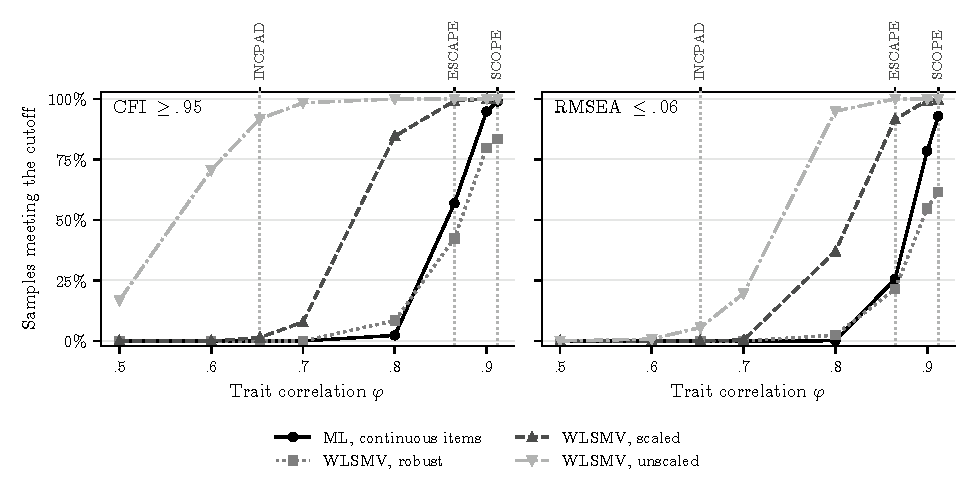
\includegraphics[width=\textwidth]{fig3.pdf}
\caption{Share of samples in which the one-factor model meets CFI $\ge .95$ (left) and RMSEA $\le .06$ (right) in the PHQ-ADS layout: 9 and 7 items with loading .75, $N = 250$. ML on continuous items, and lavaan's robust, scaled and unscaled WLSMV indices on skewed four-category items. Vertical lines mark the trait correlations of the three trials. Each point is based on 1,000 (ML) or 500 (WLSMV) replications; lines join the evaluated correlations.}
\label{fig:3}
\end{figure}

\subsection{Further Results on Loading Imbalance and Item Order}
\label{supp:imbalance}

In the setting of Figure~\ref{fig:4}, mean $|C_{\mathrm{mag}}|$ under ML was .500 at $\varphi=.2$. Under ULS, it was .834 at 0, .317 at its population threshold $1/p=.125$, .117 at .2 and .050 at .3; under WLSMV on symmetric categories, it was .037 at .2.

The unnormalized magnitude contrast showed both close agreement with the population result and attenuation at smaller sample sizes. With four items per trait, loading .7 and $N=2{,}000$, mean $|M|$ under ML at $\varphi=.2$ was .458, compared with .459 in the population. With four items per trait, loading .5 and $N=250$, it was .412 at $\varphi=0$, compared with .50 in the population. These continuous summaries describe the amount of imbalance without treating a reference distribution at one correlation as a test at another.

The effect of averaging depended on both estimator and sign convention. For continuous ML at $\varphi=0$, with four items per trait, loading .7 and $N=2{,}000$, mean $D$ and mean $|D|$ were both .701 after common sign orientation, while mean $|M|$ was .674. Opposite block signs occurred in 510 of the 1,000 fits, so the signed and magnitude contrasts cannot be interchanged. Under ULS, averaging did obscure imbalance: at its population threshold, the mean signed difference was .02 and the mean absolute difference was .30.

Among Design A fits selected by $|M|>.1$, 86\% of continuous-ML fits favored the first-listed block at $N=2{,}000$, compared with 74\% at $N=250$. The first-block/selected counts behind the directional proportions at $N=2{,}000$ in Section~\ref{sec:numerical} were 24,767/28,719 (continuous ML), 11,508/13,501 (ML on scores), 12,385/18,344 (ULS) and 2,649/4,746 (WLSMV). Each ratio pools 53 population cells, and the ordinal analyses used symmetric categories.

With the weaker block listed first, continuous ML returned a higher-objective group favoring that block in 27 to 45\% of samples with loadings .60 and .80 at $\varphi\le.01$, for $N=500$ and 2,000, compared with 94 to 100\% for loadings .68 and .72 at $\varphi\le.1$. With loadings .68 and .72, $\varphi=0$ and $N=2{,}000$, the default fit gave CFI $=.44$ and RMSEA $=.250$, compared with .56 and .223 at the best solution found, and the default factor favored the trait with lower generating loadings. Listing the weaker block last produced no weaker-block flags in any of the 234 archived cell--analysis combinations (78 population--sample-size cells $\times$ three ML analyses). Because none of the 761 replications that retained a higher-objective group under the weaker-last order had a weaker-block flag, a higher objective and a weaker-block loading pattern are distinct properties. With loadings .68 and .72 at $\varphi=.3$, above the population fold, higher-objective weaker-block groups occurred in 26\% of default fits at $N=500$ and 7\% at $N=2{,}000$. Across cells, the largest mean recorded fraction of converged random starts assigned to the selected higher-objective weaker-block group was 36\%, in a cell analyzed by ML on ordinal scores (35.5\% for continuous ML).

\subsection{Starting Covariance and Identification Controls}
\label{supp:controls}

Equal starting covariances did not imply equal optimization paths. Six population cases were refitted under two item orders and two identifications, using default starts and a common starting covariance (R 4.6.1, lavaan 0.7-2). The 48 fits included 47 reported convergences. Gradient and Hessian checks supported 39 strict local minima and identified two saddles; seven fits exceeded the gradient tolerance of $10^{-6}$. Evidence for a strict local minimum additionally required a smallest Hessian eigenvalue above $10^{-5}$.

The common starting covariance used loadings .6 and uniquenesses .64 under unit latent variance. In the unequal-loading cases, all 20 common-start fits agreed with the best numerical reference objective within $3.8\times10^{-11}$. Four exceeded the gradient tolerance, including one nonconverged fit, so objective agreement did not verify every fit as a minimum. In the exchangeable case with loading .7 and $\varphi=.3$, unit-variance identification reached the symmetric saddle, with $F=.970752$ and smallest Hessian eigenvalue $-.306480$. Marker identification reached either analytic global minimum, with $F=.940795$, depending on item order.

\subsection{Assessment of the Study Predictions}

Four predictions were stated with the design, and a fifth was added after the pilot from the categorical weighted-least-squares result. The first predicted that mean CFI and RMSEA for continuous ML would be within .01 of their population values at $N\ge1{,}000$. For Designs B and C at the best solution found, and for Design A at the default solution, RMSEA met this prediction in every evaluated cell. CFI did so except in Design A with loading .5 near $\varphi^*$, where the default-start difference reached .019 at $N=1{,}000$. Higher-objective default solutions below the fold lowered CFI by as much as .23.

The second prediction was that exchangeable designs would favor the two blocks about equally often, causing mean loadings to resemble a composite. The directional summaries did not support equal selection under the default ML start: conditional first-block proportions at $N=2{,}000$ were 86\% for ML, 85\% for ML on scores, 68\% for ULS and 56\% for WLSMV. The ordinal summaries used symmetric categories and selection required $|M|>.1$.

The third prediction was that unequal-loading designs would favor the stronger block and that weaker-block minima would occur essentially below $\varphi_f$. The best solutions found supported the stronger-block prediction. Higher-objective groups favoring the weaker block also occurred above the population fold, but these retained sample groups do not certify local minima.

The fourth prediction placed the ULS transition at $1/p$, below the ML threshold. Sample imbalance decreased across this point without disappearing. At $N=2{,}000$, mean $|C_{\mathrm{mag}}|$ was .117 at $\varphi=.2$ and .050 at .3 for ULS, compared with .500 and .312 for ML. The fifth prediction related WLSMV imbalance to its own population threshold. With four items per trait and loading .7, the population solution remained a composite; sample mean $|C_{\mathrm{mag}}|$ was .102 at $\varphi=0$ and .037 at .2 for symmetric categories and $N=2{,}000$. The diagnostics describe magnitude and polarity separately and do not define a false-positive rate by calibration at another correlation.

\section{Binary Responses}
\label{app:binary}
\label{sec:binary}

The transition from a factor favoring one trait to a factor representing both traits also appeared in population computations for binary items. We considered four normal-ogive items, two per trait, with slopes corresponding to a loading of .7. The population distribution was evaluated over all $2^p$ response patterns, and a one-trait model was fitted by minimizing KL divergence with multiple starts and 41 to 121 Gauss--Hermite nodes; the fits reported below are the best solutions found. The ratio $1-\KL/\TC$, termed information CFI, extends the population CFI interpretation to this response format.

With thresholds fixed at 0 and $\varphi=0$, the best-found fit had slopes 0 in one block and .98 in the other. The information loss was 0.0781 bits, equal to the mutual information within the ignored block, at each of 41, 81 and 121 quadrature nodes. At $\varphi=.2$, .3 and .35, the favored and other block slopes were .94 and .23, .87 and .37, and .80 and .47, respectively. At $\varphi=.4$, the slopes were equal. These computations place the binary transition between .35 and .40, below the Gaussian threshold of .49 for the corresponding design; they do not establish a general binary threshold theorem.

The information loss was almost entirely residual local dependence. Coupling the true response distribution with the fitted model's posterior distribution of the trait decomposes KL divergence into residual local dependence given the trait, item-response-function misfit, and latent-distribution misfit. The three components summed to the KL divergence within floating-point rounding (absolute difference below $10^{-15}$). Residual local dependence accounted for more than 99.5\% of the one-trait discrepancy at every evaluated $\varphi$, both with thresholds fixed at 0 and in the design of Table~\ref{tab:binary-information}.

\begin{table}[t]
\centering\small
\caption{Information retained by a one-trait normal-ogive model for four binary items generated by two correlated traits. The generating loading is .7, so the normal-ogive slope is $a=.98$; the item intercepts are $b=-.5$, .5, $-.3$ and .3 in $P(X=1\mid\theta)=\Phi(a\theta-b)$, corresponding to standardized latent-response thresholds of $-.36$, .36, $-.21$ and .21. Information is reported in bits, and the one-trait fits are the best solutions found. Sample sizes, rounded to three significant digits, use a noncentral-$\chi^2$ approximation to the full-information $G^2$ test at $\alpha=.05$, with seven degrees of freedom; finite-sample accuracy of this approximation was not assessed.}
\label{tab:binary-information}
\begin{tabular}{cccccc}
\toprule
$\varphi$ & $H(X)$, bits & $\TC(X)$, bits & KL lost by one trait, bits & Information CFI & \shortstack{Approximate $N$\\for 80\% power} \\
\midrule
.30 & 3.689 & 0.156 & 0.0545 & .651 & 190 \\
.50 & 3.663 & 0.182 & 0.0335 & .816 & 310 \\
.70 & 3.621 & 0.224 & 0.0139 & .938 & 750 \\
.80 & 3.593 & 0.251 & 0.00671 & .973 & 1,550 \\
.90 & 3.560 & 0.284 & 0.00183 & .994 & 5,660 \\
.95 & 3.541 & 0.303 & 0.000479 & .998 & 21,600 \\
\bottomrule
\end{tabular}
\end{table}

At high trait correlations, little response information distinguished the two-trait model from its one-trait approximation. Table~\ref{tab:binary-information} uses the same loading design with item intercepts $-.5$, .5, $-.3$ and .3. The response entropy was about 3.6 of the 4 possible bits. Inter-item dependence accounted for 0.16 to 0.30 bits, and the additional information lost by fitting one trait was about 0.05 bits or less. The approximate sample size for 80\% power consequently increased sharply with the trait correlation. These sample sizes use a noncentral-$\chi^2$ approximation to the full-information $G^2$ test, with seven degrees of freedom, $\alpha=.05$, and noncentrality $2N\cdot\KL$ in nats. Their finite-sample accuracy, including behavior near transition points or nonregular endpoints, was not assessed.

\end{document}
